% tugas_data_analitik.tex
% Laporan Tugas Data Analitik — C-MAPSS RUL Prediction (Complete Version)
% Departemen Teknik Mesin FTUI — 2026

\documentclass[11pt,a4paper]{article}

\usepackage[T1]{fontenc}
\usepackage[utf8]{inputenc}
\usepackage[a4paper, margin=2.5cm]{geometry}
\usepackage{setspace}
\usepackage{parskip}
\usepackage{titlesec}
\usepackage{fancyhdr}
\usepackage{booktabs}
\usepackage{tabularx}
\usepackage{multirow}
\usepackage{graphicx}
\usepackage{caption}
\usepackage{subcaption}
\usepackage{xcolor}
\usepackage{amsmath}
\usepackage{amssymb}
\usepackage{hyperref}
\usepackage{enumitem}
\usepackage{float}
\usepackage{tocloft}
\usepackage{url}

\definecolor{uiblue}{RGB}{0,56,147}
\definecolor{mygray}{RGB}{100,100,100}

\titleformat{\section}
  {\large\bfseries\color{uiblue}}
  {\thesection}{0.6em}{}[\vspace{2pt}\hrule\vspace{4pt}]
\titleformat{\subsection}
  {\normalsize\bfseries\color{uiblue}}{\thesubsection}{0.6em}{}
\titleformat{\subsubsection}
  {\small\bfseries}{\thesubsubsection}{0.6em}{}

\pagestyle{fancy}
\fancyhf{}
\fancyhead[L]{\small\color{mygray}
  Tugas Data Analitik -- Prediksi RUL Mesin Turbofan C-MAPSS}
\fancyhead[R]{\small\color{mygray} Data Analitik 2026}
\fancyfoot[C]{\small\color{mygray}\thepage}
\renewcommand{\headrulewidth}{0.4pt}
\renewcommand{\footrulewidth}{0.0pt}

\onehalfspacing
\captionsetup{font=small, labelfont=bf}
\hypersetup{colorlinks=true, linkcolor=uiblue,
            urlcolor=uiblue, citecolor=uiblue}

% ══════════════════════════════════════════════════════════════════════════════
\begin{document}

% ── Cover ─────────────────────────────────────────────────────────────────────
\begin{titlepage}
  \centering
  \vspace*{1.0cm}
  
\includegraphics[width=2.2cm]{images/logo_ui.png}
  \vspace{0.6cm}

  {\large\bfseries UNIVERSITAS INDONESIA\par}
  \vspace{0.2cm}
  {\normalsize Fakultas Teknik -- Departemen Teknik Mesin\par}

  \vspace{0.5cm}
  \hrule height 1.2pt
  \vspace{0.4cm}
  {\LARGE\bfseries\color{uiblue}
    PREDIKSI \textit{REMAINING USEFUL LIFE}\\[0.3em]
    MESIN TURBOFAN MENGGUNAKAN\\[0.3em]
    \textit{ARTIFICIAL NEURAL NETWORK}\\[0.3em]
    PADA DATASET C-MAPSS\par}
  \vspace{0.4cm}
  \hrule height 1.2pt

  \vspace{1.0cm}
  {\normalsize\color{mygray} Mata Kuliah:\par}
  {\large\bfseries Data Analitik\par}
  \vspace{0.6cm}
  {\normalsize\color{mygray} Dosen Pengampu:\par}
  {\normalsize Dr.\ Eng.\ Sholahudin, S.T., M.Sc.\par}

  \vspace{0.8cm}
  {\normalsize\color{mygray} Disusun Oleh:\par}
  \vspace{0.4cm}
  \begin{tabular}{ll}
    2506565466 & Luqman Alifio Arhab \\[4pt]
    2506565414 & Azfa Rhazasta Abiandra \\[4pt]
    2506565401 & Adamsyah Haryo Saksono \\[4pt]
    2506565433 & Epsiarto Rizqi Nurwijayadi \\[4pt]
  \end{tabular}

  \vspace{0.2cm}
  \vfill
  {\normalsize\bfseries
    DEPARTEMEN TEKNIK MESIN\\
    FAKULTAS TEKNIK\\
    UNIVERSITAS INDONESIA\\[0.4em]
    2026\par}
\end{titlepage}

\thispagestyle{empty}
\newpage
\setcounter{page}{1}
\tableofcontents
\newpage

% ══════════════════════════════════════════════════════════════════════════════
\section{Pendahuluan}

\subsection{Latar Belakang}

Prediksi \textit{Remaining Useful Life} (RUL) merupakan komponen kunci dalam
sistem \textit{Prognostics and Health Management} (PHM). Dengan mengetahui
sisa umur pakai komponen sebelum kegagalan, jadwal perawatan dapat
dioptimalkan sehingga mengurangi biaya \textit{downtime} tak terencana dan
risiko kegagalan mendadak yang berpotensi berbahaya.

\begin{figure}[H]
  \centering
  
\includegraphics[width=0.58\textwidth]{images/01_phm_ecosystem_stack.png}
  \caption{Hierarki PHM --- laporan ini berfokus pada lapisan
    \textit{Prognostics} (prediksi RUL), lapisan kedua dari atas}
  \label{fig:phm}
\end{figure}

Sistem PHM terdiri dari beberapa lapisan mulai dari \textit{sensing}
(pengumpulan data sensor) hingga \textit{decision making} (perencanaan
perawatan). Laporan ini berfokus pada lapisan \textbf{Prognostics} ---
menjawab pertanyaan ``berapa lama lagi komponen ini akan bertahan?''

Pada mesin turbofan penerbangan, degradasi komponen seperti
\textit{High Pressure Compressor} (HPC) dan \textit{Fan} berlangsung
secara gradual dan tercermin dalam perubahan pola sensor.
Tantangan utamanya adalah memisahkan sinyal degradasi dari variasi
kondisi operasi yang normal.

\subsection{Tujuan}

\begin{enumerate}[noitemsep]
  \item Membersihkan data dengan analisis korelasi sensor terhadap output (RUL)
  \item Menormalisasi data dengan metode \textit{z-score} berbasis siklus sehat
  \item Memilih fitur menggunakan korelasi Pearson dan PCA
  \item Membangun dan membandingkan model MLP pada empat sub-dataset
  \item Menganalisis kepentingan fitur dengan algoritma Garson
\end{enumerate}

\subsection{Alur Pipeline}

\begin{figure}[H]
  \centering\small
  \begin{tabular}{ccccc}
    \fbox{Raw .txt NASA} & $\rightarrow$ &
    \fbox{HDF5} & $\rightarrow$ &
    \fbox{Cleaning} \\[6pt]
    & & & & $\downarrow$ \\[2pt]
    \fbox{Garson} & $\leftarrow$ &
    \fbox{ANN} & $\leftarrow$ &
    \fbox{Normalisasi + PCA}
  \end{tabular}
  \caption{Alur pipeline analitik lengkap}
  \label{fig:pipeline}
\end{figure}

% ══════════════════════════════════════════════════════════════════════════════
\section{Dataset C-MAPSS}

\subsection{Deskripsi Dataset}

Dataset C-MAPSS (\textit{Commercial Modular Aero-Propulsion System Simulation})
dipublikasikan oleh NASA \cite{saxena2008} dan tersedia di:
\begin{center}
  \small\url{https://www.nasa.gov/intelligent-systems-division/discovery-and-systems-health/pcoe/pcoe-data-set-repository/}
\end{center}

\begin{figure}[H]
  \centering
  
\includegraphics[width=0.90\textwidth]{images/09_dataset_matrix.png}
  \caption{Matriks karakteristik empat sub-dataset C-MAPSS ---
    FD001 (termudah: 1 kondisi, 1 mode kerusakan) hingga FD004
    (tersulit: 6 kondisi, 2 mode kerusakan)}
  \label{fig:dataset_matrix}
\end{figure}

Empat sub-dataset tersedia dengan tingkat kompleksitas berbeda.
FD001 dan FD003 memiliki satu kondisi operasi (sea level),
sedangkan FD002 dan FD004 memiliki enam kondisi operasi berbeda
(altitude, Mach number, throttle resolver angle).
Mode kerusakan HPC terdapat di semua sub-dataset;
FD003 dan FD004 menambahkan kerusakan Fan secara bersamaan.

\subsection{Struktur Mesin dan Sensor}

\begin{figure}[H]
  \centering
  
\includegraphics[width=0.88\textwidth]{images/03_cmapss_engine_schematic.png}
  \caption{Skema mesin turbofan C-MAPSS --- 21 sensor mengukur kondisi
    di sepanjang aliran udara dari inlet hingga exhaust;
    HPC adalah komponen yang mengalami degradasi pada semua sub-dataset}
  \label{fig:engine}
\end{figure}

Setiap baris data terdiri dari 26 kolom tanpa \textit{header}:
\texttt{unit\_number}, \texttt{time\_cycles}, tiga \textit{op\_settings},
dan 21 sensor. Sensor mengukur suhu, tekanan, kecepatan poros, dan aliran
udara di berbagai titik sepanjang mesin.

\subsection{Konsep RUL dan Struktur File}

\begin{figure}[H]
  \centering
  
\includegraphics[width=0.85\textwidth]{images/10_train_test_rul_relationship.png}
  \caption{Hubungan antara file train, test, dan RUL ---
    data \textit{train} mencatat siklus penuh hingga kegagalan
    sehingga RUL dapat dihitung langsung;
    data \textit{test} dipotong di siklus $t^*$ dan
    \texttt{RUL\_FDxxx.txt} berisi kunci jawaban}
  \label{fig:rul_rel}
\end{figure}

Data \textit{train} mencatat siklus penuh hingga kegagalan sehingga
RUL dapat dihitung: $\text{RUL} = t_{\max} - t_{\text{saat ini}}$.
Data \textit{test} dipotong sebelum kegagalan --- ini adalah kondisi
\textit{deployment} nyata di mana kita tidak tahu kapan mesin akan gagal.
File \texttt{RUL\_FDxxx.txt} berisi satu integer per mesin test sebagai
kunci jawaban untuk evaluasi model.

\subsection{Motivasi: Mengapa Prediksi RUL Sulit}

\begin{figure}[H]
  \centering
  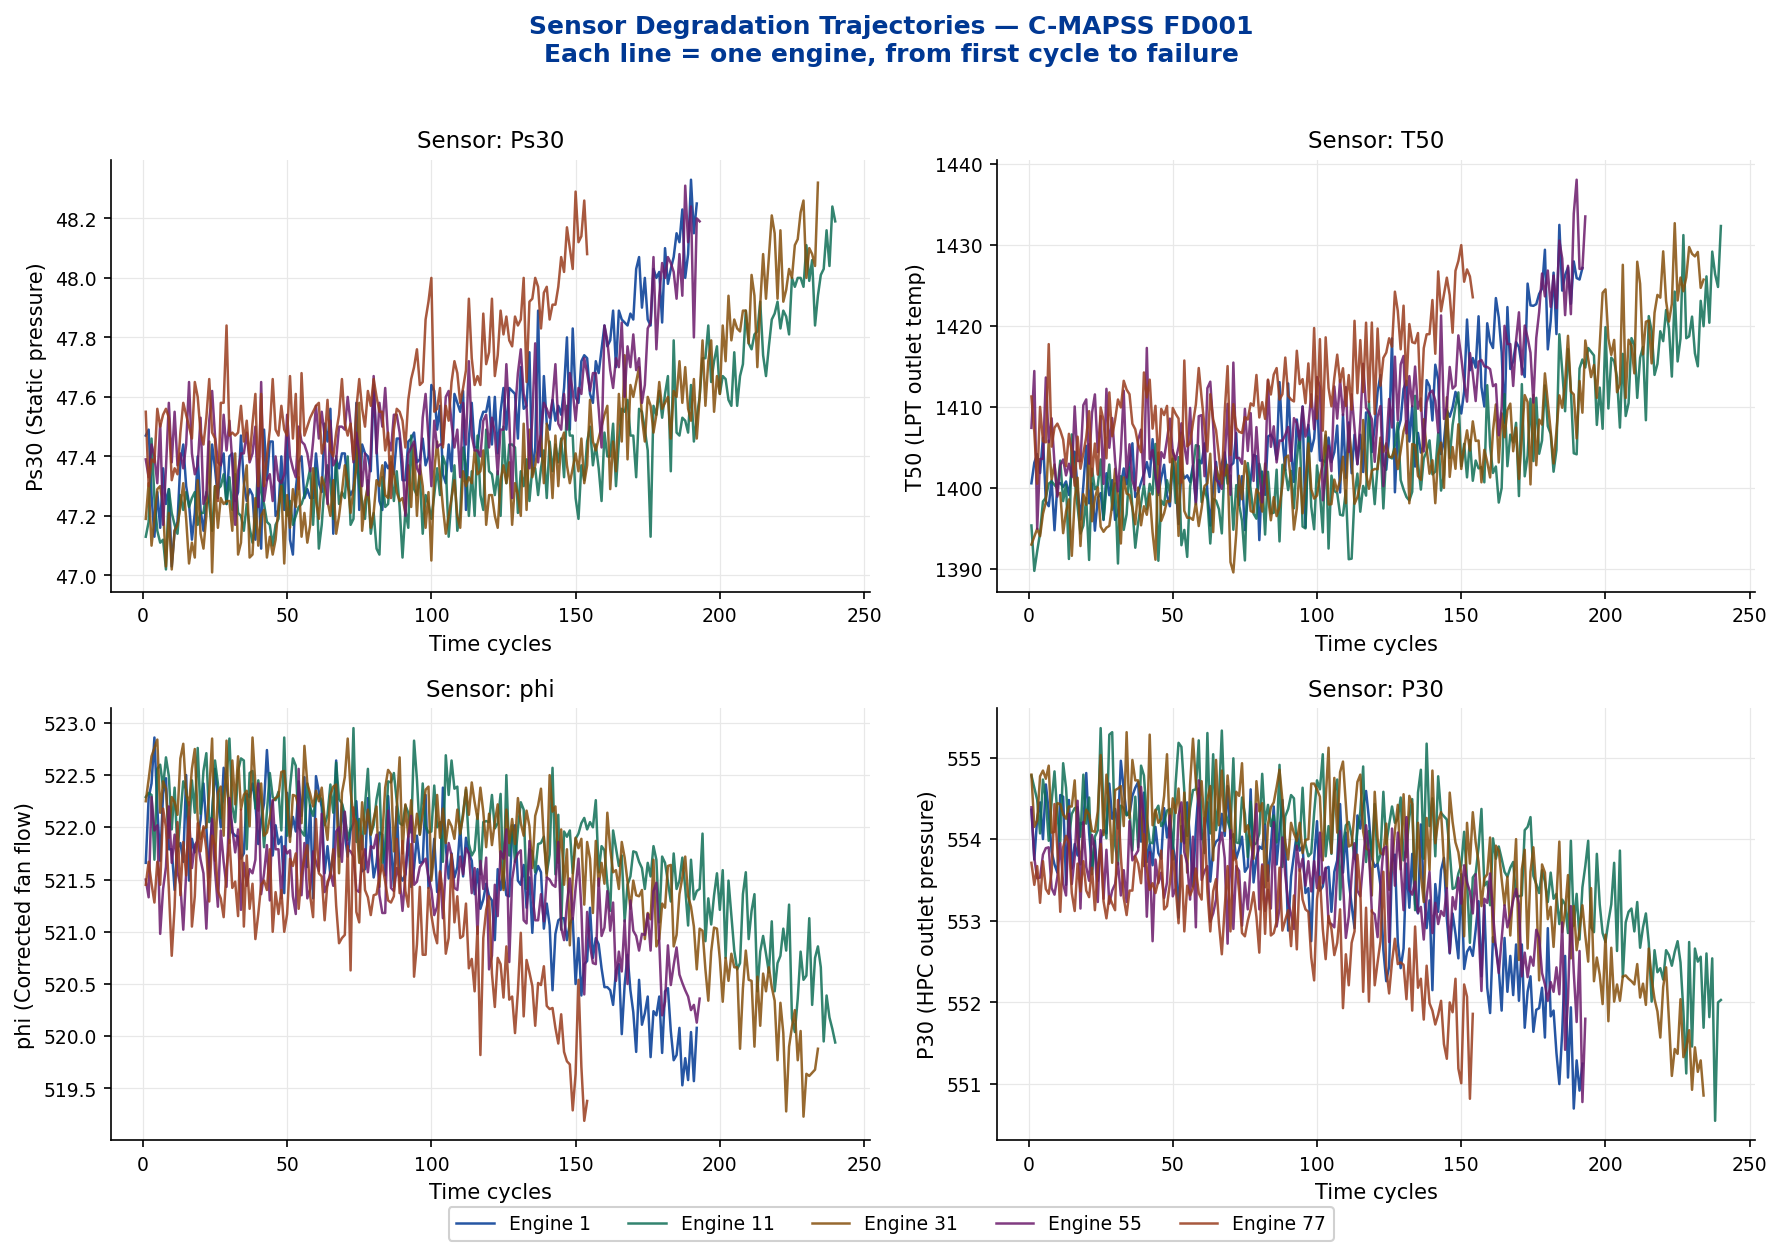
\includegraphics[width=0.95\textwidth]{images/plot_A1_degradation.png}
  \caption{Trajektori degradasi sensor FD001 untuk lima mesin representatif ---
    setiap garis adalah satu mesin dari siklus pertama hingga kegagalan;
    sensor Ps30, T50, phi, dan P30 menunjukkan drift yang jelas
    menjelang akhir umur mesin}
  \label{fig:degradation}
\end{figure}

Gambar \ref{fig:degradation} menunjukkan mengapa prediksi RUL adalah masalah
yang tidak trivial. Setiap mesin memiliki umur total berbeda (x-axis berakhir
di titik berbeda). Sensor mulai dengan nilai yang relatif stabil di fase sehat,
kemudian mulai menyimpang secara gradual di fase degradasi. Penyimpangan
inilah yang harus dipelajari model untuk memprediksi berapa siklus tersisa.

\subsection{Struktur HDF5}

Seluruh data disimpan dalam format HDF5 menggunakan satu skrip konsolidasi
\texttt{build\_cmapss\_complete.py} yang membaca langsung dari file \texttt{.txt}
NASA tanpa file perantara.

\begin{figure}[H]
  \centering
  \begin{subfigure}[b]{0.30\textwidth}
    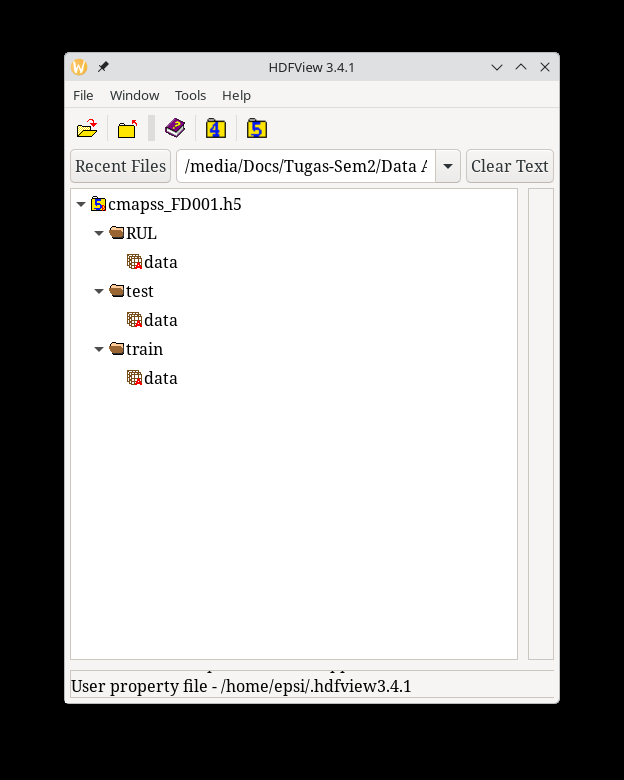
\includegraphics[width=\textwidth]{images/hdf5-01-vanilla-01-main.png}
    \caption{Vanilla HDF5}
  \end{subfigure}
  \hfill
  \begin{subfigure}[b]{0.30\textwidth}
    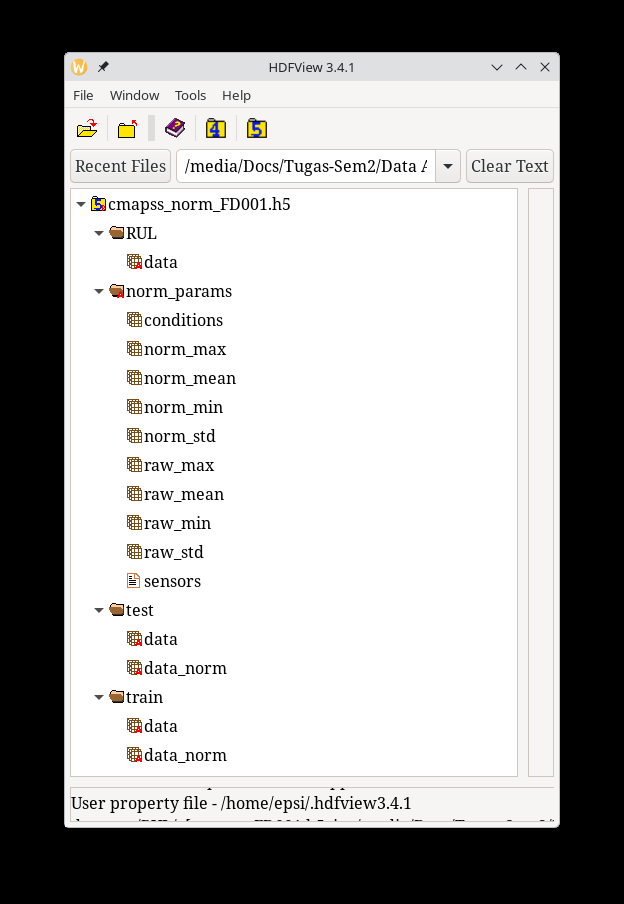
\includegraphics[width=\textwidth]{images/hdf5-03-normal-01-main.png}
    \caption{+ Normalisasi}
  \end{subfigure}
  \hfill
  \begin{subfigure}[b]{0.30\textwidth}
    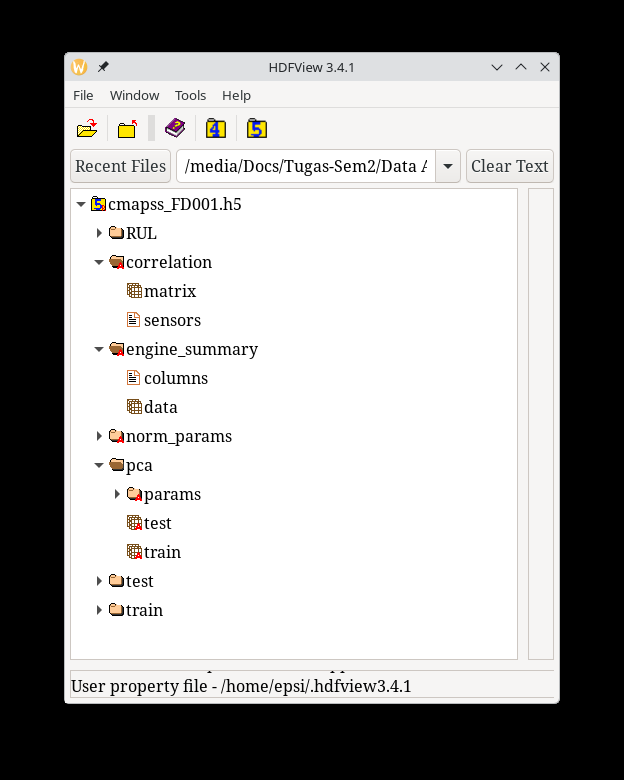
\includegraphics[width=\textwidth]{images/hdf5-05-pca-01-main.png}
    \caption{+ Korelasi + PCA}
  \end{subfigure}
  \caption{Evolusi struktur HDF5 dari vanilla hingga lengkap}
  \label{fig:hdf5_evolution}
\end{figure}

% ══════════════════════════════════════════════════════════════════════════════
\section{Pembersihan Data}

\subsection{Metode}

Pembersihan data dilakukan dengan menganalisis korelasi setiap sensor
terhadap output (RUL). Sensor yang tidak membawa informasi degradasi
dieliminasi menggunakan lima metode statistik secara bersamaan:

\begin{enumerate}[noitemsep]
  \item \textbf{Standar Deviasi (std)} --- sensor konstan (std $= 0$)
    tidak bervariasi sama sekali
  \item \textbf{Koefisien Variasi (CV)} --- $\text{CV} = \sigma/|\mu|$;
    nilai sangat kecil menunjukkan variasi tidak signifikan
  \item \textbf{Korelasi Pearson vs RUL} --- mengukur hubungan \textit{linear}
    sensor terhadap output; nilai $\approx 0$ berarti tidak ada hubungan linear
  \item \textbf{Korelasi Spearman vs RUL} --- mengukur hubungan
    \textit{monoton}; lebih robust terhadap non-linearitas
  \item \textbf{Mutual Information (MI) vs RUL} --- menangkap hubungan
    non-linear; nilai $\approx 0$ berarti tidak ada hubungan sama sekali
\end{enumerate}

\subsection{Hasil Analisis FD001}

\begin{table}[H]
\centering\small
\caption{Statistik sensor FD001 terhadap output RUL ---
  sensor dengan std $= 0$ ditandai ($\dagger$)}
\label{tab:sensor_stats}
\begin{tabular}{lrrrrrrl}
\toprule
Sensor & Mean & Std & CV & Pearson & Spearman & MI & Hapus \\
\midrule
T2$^\dagger$         & 518.67 & 0.000 & 0.000 & NaN     & NaN     & 0.000 & \checkmark \\
T24          & 642.68 & 0.500 & 0.001 & $-$0.607 & $-$0.629 & 0.342 & \\
T30          & 1590.5 & 6.131 & 0.004 & $-$0.585 & $-$0.606 & 0.306 & \\
T50          & 1408.9 & 9.001 & 0.006 & $-$0.679 & $-$0.702 & 0.467 & \\
P2$^\dagger$         &  14.62 & 0.000 & 0.000 & NaN     & NaN     & 0.006 & \checkmark \\
P15          &  21.61 & 0.001 & 0.000 & $-$0.128 & $-$0.128 & 0.006 & \checkmark \\
P30          & 553.37 & 0.885 & 0.002 & $+$0.657 & $+$0.679 & 0.425 & \\
Nf           & 2388.1 & 0.071 & 0.000 & $-$0.564 & $-$0.574 & 0.258 & \\
Nc           & 9065.2 & 22.08 & 0.002 & $-$0.390 & $-$0.322 & 0.222 & \\
epr$^\dagger$        &   1.30 & 0.000 & 0.000 & NaN     & NaN     & 0.000 & \checkmark \\
Ps30         &  47.54 & 0.267 & 0.006 & $-$0.696 & $-$0.718 & 0.507 & \\
phi          & 521.41 & 0.738 & 0.001 & $+$0.672 & $+$0.693 & 0.442 & \\
NRf          & 2388.1 & 0.072 & 0.000 & $-$0.563 & $-$0.573 & 0.262 & \\
NRc          & 8143.8 & 19.08 & 0.002 & $-$0.307 & $-$0.202 & 0.225 & \\
BPR          &   8.44 & 0.038 & 0.004 & $-$0.643 & $-$0.666 & 0.390 & \\
farB$^\dagger$       &   0.03 & 0.000 & 0.000 & NaN     & NaN     & 0.000 & \checkmark \\
htBleed      & 393.21 & 1.549 & 0.004 & $-$0.606 & $-$0.629 & 0.328 & \\
Nf\_dmd$^\dagger$    & 2388.0 & 0.000 & 0.000 & NaN     & NaN     & 0.000 & \checkmark \\
PCNfR\_dmd$^\dagger$ & 100.00 & 0.000 & 0.000 & NaN     & NaN     & 0.000 & \checkmark \\
W31          &  38.82 & 0.181 & 0.005 & $+$0.629 & $+$0.653 & 0.367 & \\
W32          &  23.29 & 0.108 & 0.005 & $+$0.636 & $+$0.657 & 0.380 & \\
\bottomrule
\multicolumn{8}{l}{\small $^\dagger$ std $= 0$:
  Pearson/Spearman tidak terdefinisi (NaN); dieliminasi}
\end{tabular}
\end{table}

Sensor dengan std $= 0$ menghasilkan nilai Pearson dan Spearman
\texttt{NaN} --- bukti matematis paling kuat bahwa sensor tersebut
tidak dapat berkorelasi dengan apapun. Sensor P15 dieliminasi karena
CV $\approx 0$ dan Pearson hanya $-0{,}13$ (hampir tidak ada korelasi
dengan RUL).

\subsection{Perbandingan Antar Sub-dataset}

\begin{table}[H]
\centering\small
\caption{Sensor yang dieliminasi per sub-dataset}
\label{tab:drop}
\begin{tabular}{lcp{8.5cm}}
\toprule
Sub-dataset & Dihapus & Sensor \\
\midrule
FD001 & 6 & T2, P2, epr, farB, Nf\_dmd, PCNfR\_dmd \\
FD002 & 0 & (tidak ada --- semua sensor bervariasi antar 6 kondisi operasi) \\
FD003 & 5 & T2, P2, farB, Nf\_dmd, PCNfR\_dmd \\
FD004 & 0 & (tidak ada) \\
\bottomrule
\end{tabular}
\end{table}

FD002 dan FD004 tidak mengeliminasi sensor apapun karena variasi antar
6 kondisi operasi membuat semua sensor bervariasi. Sensor seperti T2
bersifat konstan dalam satu kondisi (FD001) namun bervariasi antar
kondisi (FD002). FD003 mempertahankan \texttt{epr} karena memiliki
std $= 0{,}0035$ --- kecil namun tidak nol --- akibat mode kerusakan
HPC+Fan yang berbeda dari FD001.

% ══════════════════════════════════════════════════════════════════════════════
\section{Normalisasi}

\subsection{Metode Z-Score Berbasis Siklus Sehat}

\begin{figure}[H]
  \centering
  
\includegraphics[width=0.82\textwidth]{images/13_normalization_pipeline.png}
  \caption{Pipeline normalisasi per kondisi --- parameter $\mu_c$ dan $\sigma_c$
    dihitung dari siklus sehat (RUL\_raw $\geq 125$) lalu diterapkan
    ke seluruh data termasuk siklus terdegradasi}
  \label{fig:norm_pipeline}
\end{figure}

Normalisasi menggunakan formula \textit{z-score}:
\begin{equation}
  z = \frac{x - \mu_{c,\,\text{healthy}}}{\sigma_{c,\,\text{healthy}}}
  \label{eq:zscore}
\end{equation}

di mana $\mu_c$ dan $\sigma_c$ dihitung hanya dari siklus dengan
RUL\_raw $\geq 125$ (\textit{healthy cycles}) untuk kondisi operasi $c$.

\subsection{Mengapa Siklus Sehat Saja}

\begin{figure}[H]
  \centering
  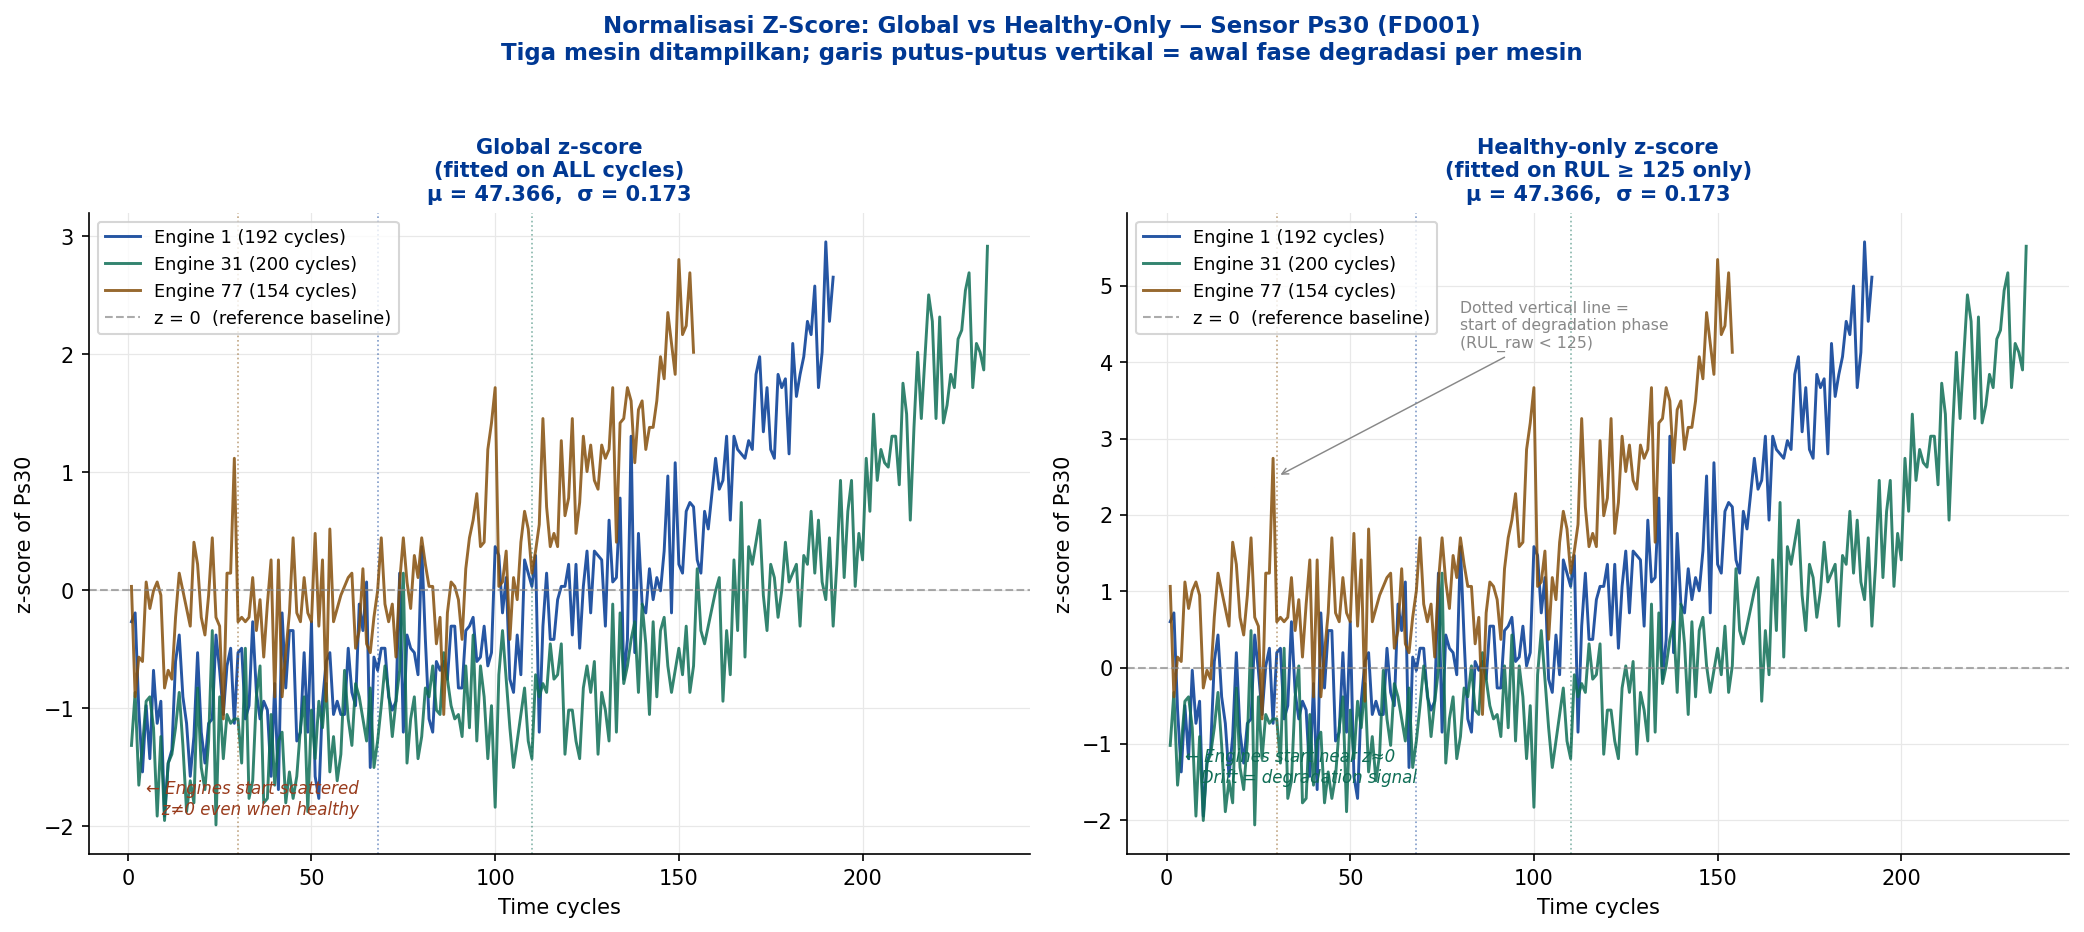
\includegraphics[width=0.96\textwidth]{images/plot_D13_norm_comparison.png}
  \caption{Perbandingan normalisasi global vs \textit{healthy-only} untuk
    sensor Ps30 pada tiga mesin (Engine 1, 31, 77) FD001 ---
    garis putus-putus vertikal menandai awal fase degradasi per mesin
    (saat RUL\_raw turun di bawah 125)}
  \label{fig:norm_comparison}
\end{figure}

Gambar \ref{fig:norm_comparison} menunjukkan perbedaan kedua metode
pada sensor Ps30 untuk tiga mesin sekaligus. Setiap garis berwarna
merepresentasikan satu mesin: Engine 1 (biru, 192 siklus), Engine 31
(hijau, $\approx$200 siklus), dan Engine 77 (coklat, 154 siklus).
Garis putus-putus vertikal menandai kapan fase degradasi dimulai
untuk masing-masing mesin.

\textbf{Global z-score (kiri)}: ketiga mesin mulai pada nilai z yang
tersebar ($-1$ hingga $+1$). Artinya, mesin yang sehat pun sudah
memiliki z $\neq 0$ hanya karena $\mu$ dipengaruhi oleh siklus
terdegradasi di seluruh dataset. Referensi nol tidak merepresentasikan
kondisi sehat.

\textbf{Healthy-only z-score (kanan)}: ketiga mesin mulai mendekati
$z \approx 0$ di siklus awal, lalu secara konsisten \textit{drift}
ke atas seiring degradasi. Penyimpangan dari nol adalah sinyal
degradasi yang akan dipelajari model ANN.

\subsection{Mengapa Per Kondisi, Bukan Global}

Pada FD002 dan FD004 terdapat 6 kondisi operasi. Sensor seperti T2
bernilai $\approx 518$\,R pada kondisi 1 namun $\approx 445$\,R pada
kondisi lain --- selisih 73\,R ini bukan degradasi, melainkan perbedaan
kondisi operasi. Normalisasi global akan mengaburkan sinyal degradasi
dengan variasi kondisi. Normalisasi per kondisi menghilangkan efek
kondisi terlebih dahulu, menyisakan hanya sinyal degradasi.

\subsection{Penerapan ke Data Test}

Data \textit{test} dinormalisasi menggunakan parameter dari data
\textit{train}:
\begin{equation}
  z_{\text{test}} =
  \frac{x_{\text{test}} - \mu_{c,\,\text{train,\,healthy}}}
       {\sigma_{c,\,\text{train,\,healthy}}}
\end{equation}

Menggunakan parameter \textit{test} sendiri merupakan \textit{data leakage}
karena pada kondisi \textit{deployment} nyata, distribusi data masa
depan tidak diketahui saat pelatihan.

% ══════════════════════════════════════════════════════════════════════════════
\section{Seleksi Fitur}

\subsection{Korelasi Pearson Antar Sensor}

\begin{figure}[H]
  \centering
  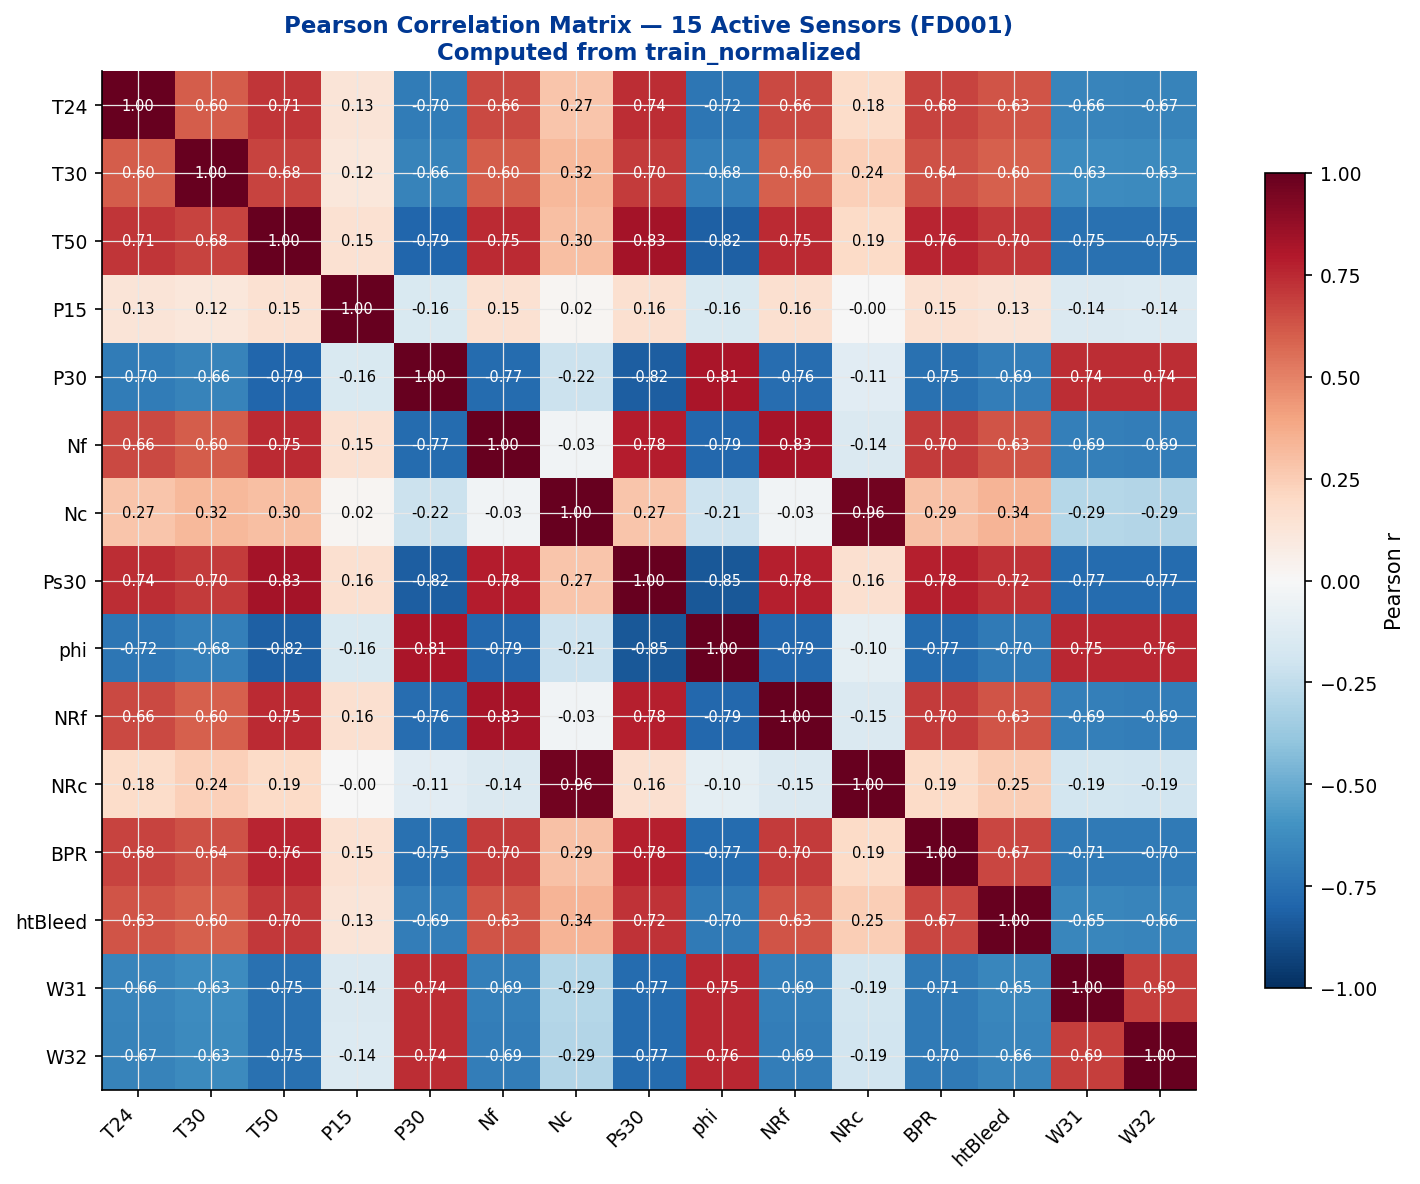
\includegraphics[width=0.82\textwidth]{images/plot_A2_correlation.png}
  \caption{Matriks korelasi Pearson antar 15 sensor aktif (FD001,
    dihitung dari \texttt{train\_normalized}) ---
    sel putih = sensor konstan yang dieliminasi;
    blok merah gelap menunjukkan pasangan sensor yang sangat
    berkorelasi (Nc--NRc $r = 0{,}96$, Nf--NRf $r = 0{,}83$)}
  \label{fig:corr}
\end{figure}

Gambar \ref{fig:corr} menunjukkan matriks korelasi Pearson.
Sel putih adalah baris/kolom sensor yang dieliminasi (std $= 0$).
Blok merah gelap pada pasangan Nc--NRc ($r = 0{,}96$) dan
Nf--NRf ($r = 0{,}83$) menunjukkan redundansi tinggi ---
kedua sensor dalam pasangan tersebut membawa informasi yang hampir
identik. Inilah motivasi utama penggunaan PCA: membuang redundansi
sambil mempertahankan informasi.

\subsection{Principal Component Analysis (PCA)}

\subsubsection{Varians yang Dijelaskan}

\begin{figure}[H]
  \centering
  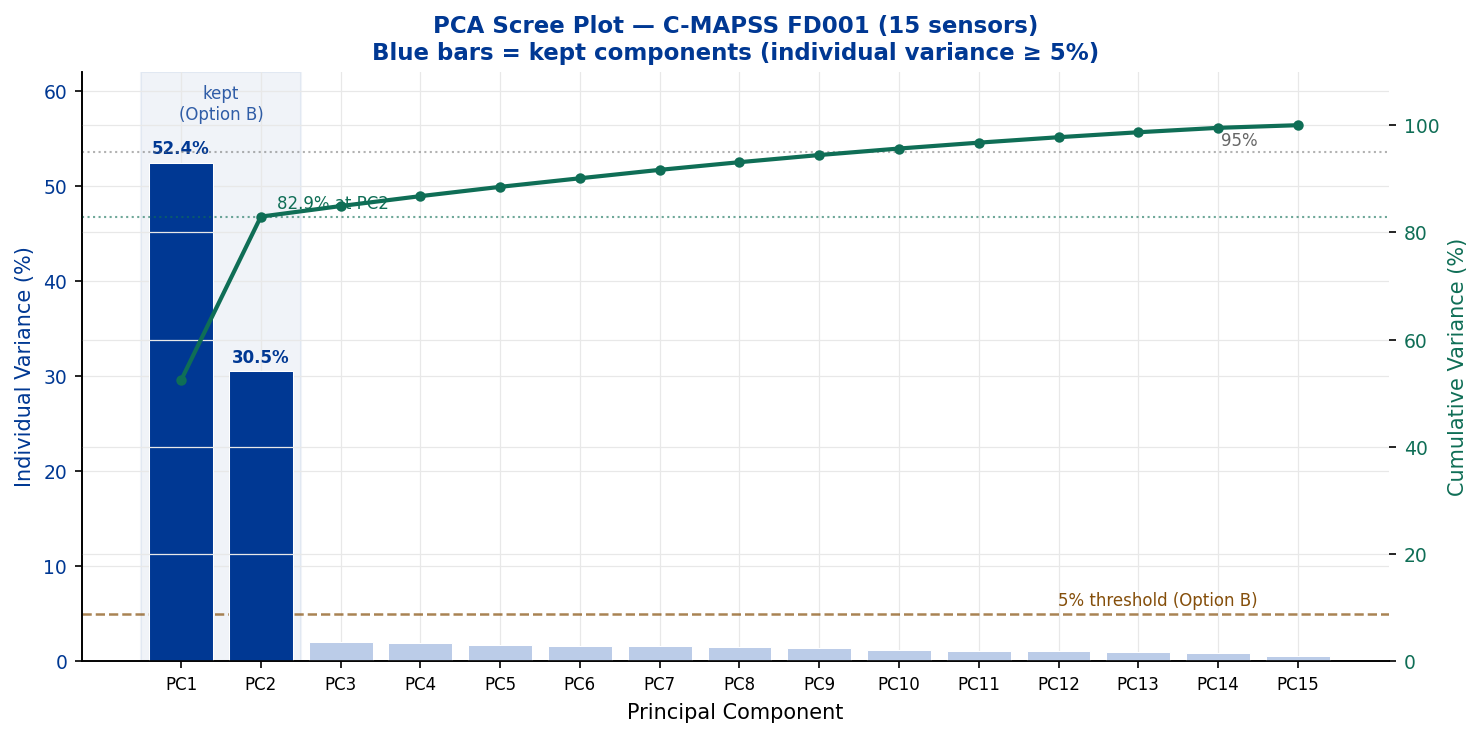
\includegraphics[width=0.88\textwidth]{images/plot_A3_scree.png}
  \caption{\textit{Scree plot} PCA FD001 (15 sensor) ---
    batang biru = komponen yang dipertahankan (varians individual
    $\geq 5\%$); garis teal = varians kumulatif;
    \textit{cliff} setelah PC2 menunjukkan PC3 dan seterusnya
    hanya mengandung \textit{noise}}
  \label{fig:scree}
\end{figure}

Gambar \ref{fig:scree} menunjukkan \textit{scree plot} --- grafik
varians individual per komponen. Terdapat \textit{scree cliff} yang
sangat tajam setelah PC2: PC1 = 52,4\%, PC2 = 30,5\%, kemudian
PC3 tiba-tiba turun ke 2,0\%. Ini berarti hampir semua informasi
bermakna sudah terangkum dalam dua komponen pertama. Komponen
PC3 dan seterusnya sebagian besar merupakan \textit{noise} sisa.

\begin{table}[H]
\centering\small
\caption{Ringkasan PCA per sub-dataset (Opsi B: varians $\geq 5\%$)}
\label{tab:pca_kept}
\begin{tabular}{lcccl}
\toprule
Sub-dataset & Sensor & Komponen & Varians Kumulatif & Komponen Dominan \\
\midrule
FD001 & 15 & 2 & 82,9\% & PC1: speed (52,4\%), PC2: pressure contrast \\
FD002 & 21 & 4 & 74,8\% & PC1: speed (41,6\%), PC3: epr alone (8,4\%) \\
FD003 & 16 & 3 & 87,8\% & PC1: speed (60,2\%) \\
FD004 & 21 & 3 & 77,5\% & PC1: speed (48,4\%) \\
\bottomrule
\end{tabular}
\end{table}

\subsubsection{Interpretasi PCA dalam Ruang 2D}

\begin{figure}[H]
  \centering
  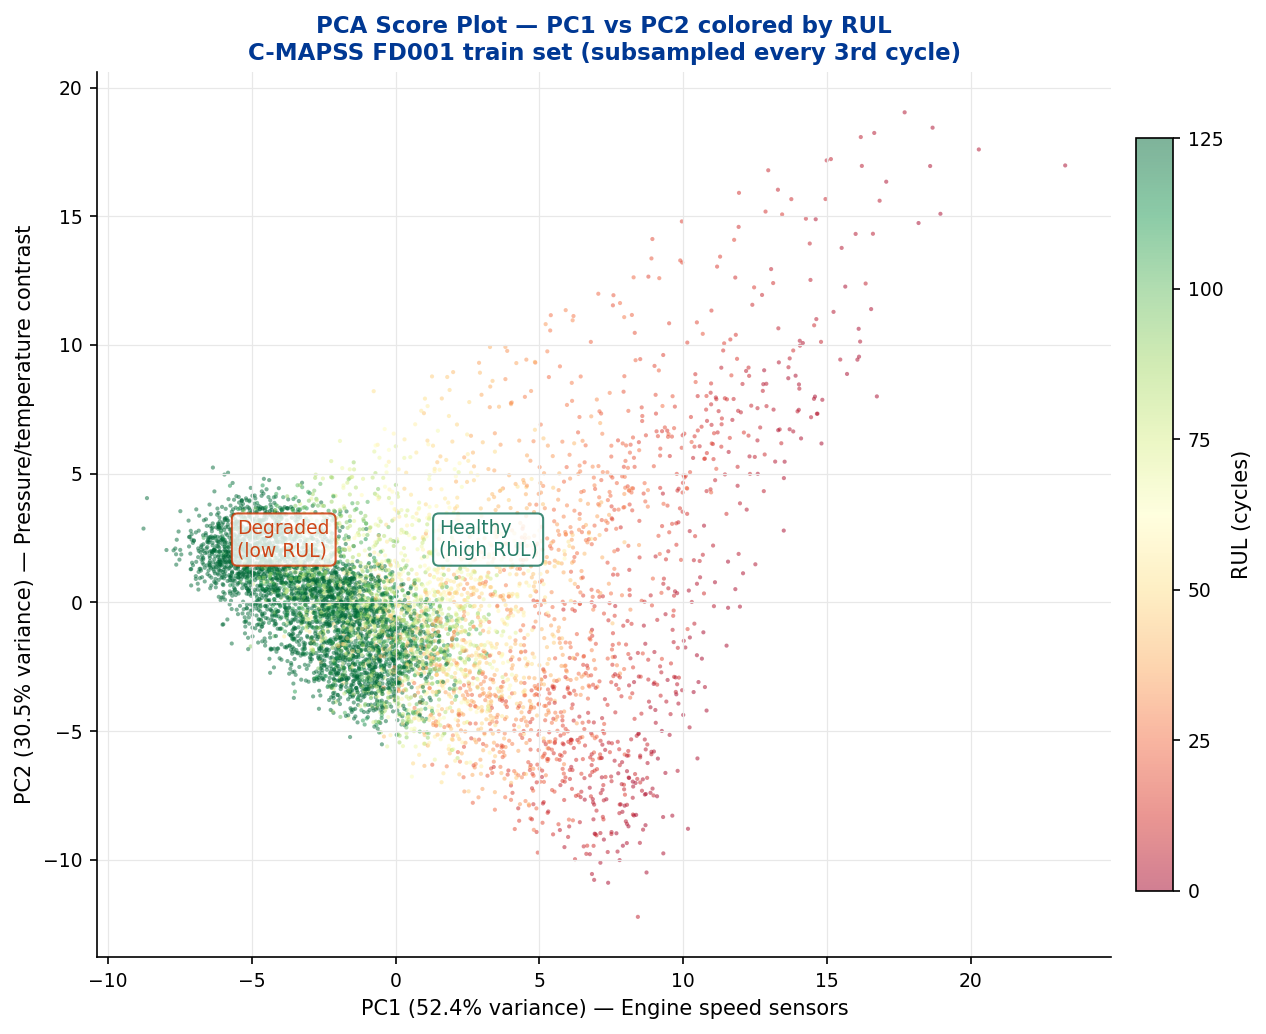
\includegraphics[width=0.82\textwidth]{images/plot_A4_pca_scatter.png}
  \caption{\textit{Scatter plot} PC1 vs PC2 diwarnai berdasarkan nilai RUL ---
    hijau = sehat (RUL tinggi), merah = mendekati gagal (RUL rendah);
    setiap titik adalah satu siklus mesin dari data \textit{train}
    FD001 (disubsampel setiap 3 siklus untuk keterbacaan)}
  \label{fig:pca_scatter}
\end{figure}

Gambar \ref{fig:pca_scatter} menunjukkan seluruh data \textit{train}
FD001 yang sudah dikompresi menjadi 2 angka (PC1 dan PC2) per siklus.
Setiap titik adalah satu siklus operasi satu mesin. Warna merepresentasikan
RUL sebagai dimensi ketiga (pseudo-3D).

Pola yang terlihat: titik-titik hijau (mesin sehat, RUL tinggi) cenderung
berada di sisi kanan (PC1 positif), sedangkan titik-titik merah (mendekati
kegagalan, RUL rendah) berada di sisi kiri (PC1 negatif). Ini membuktikan
PC1 memang menangkap sinyal degradasi --- mesin yang terdegradasi memiliki
nilai PC1 yang berbeda dari mesin sehat.

\subsubsection{Interpretasi Eigenvectors}

\begin{figure}[H]
  \centering
  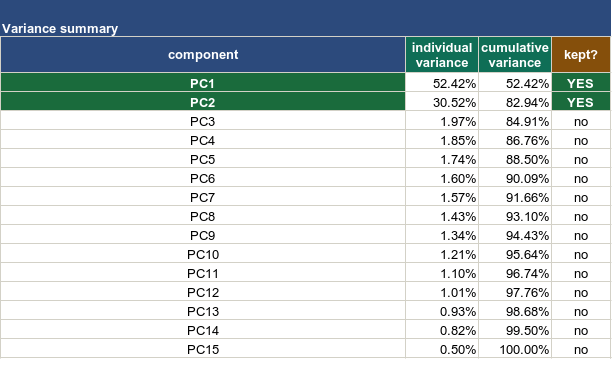
\includegraphics[width=0.80\textwidth]{images/spreadsheet-06-pca-11a-pca-params.png}
  \caption{Tabel varians dan matriks \textit{eigenvectors} pada spreadsheet
    v6 (FD002) --- PC3 didominasi oleh \texttt{epr} dengan
    \textit{loading} 0,94, mengisolasinya menjadi komponen tersendiri}
  \label{fig:pca_params}
\end{figure}

Interpretasi fisik komponen FD001:
\begin{itemize}[noitemsep]
  \item \textbf{PC1} (52,4\%): didominasi Nf, NRf, Nc, NRc ---
    sensor kecepatan poros; merepresentasikan
    \textit{overall engine speed state}
  \item \textbf{PC2} (30,5\%): kontras antara sensor kecepatan (positif)
    dan sensor tekanan/suhu (negatif) ---
    merepresentasikan \textit{compressor loading condition}
\end{itemize}

\subsection{Pipeline Spreadsheet}

\begin{table}[H]
\centering\small
\caption{Evolusi spreadsheet v3--v6 dan sheet yang ditambahkan}
\label{tab:spreadsheet}
\begin{tabular}{llp{9cm}}
\toprule
Versi & Sheet Baru & Isi \\
\midrule
v3 & train, test, RUL
   & Data raw + kolom komputasi (condition\_id, dT, RUL\_raw, dll.) \\
v4 & train\_normalized
   & Sensor ternormalisasi (z-score per kondisi, healthy-only) \\
v5 & test\_normalized, stats, correlation, engine\_summary
   & Normalisasi test, statistik per sensor, korelasi, ringkasan mesin \\
v6 & pca\_params, pca\_train, pca\_test
   & Parameter PCA (eigenvectors, varians) + skor PC per siklus \\
\bottomrule
\end{tabular}
\end{table}

\begin{figure}[H]
  \centering
  \begin{subfigure}[b]{0.48\textwidth}
    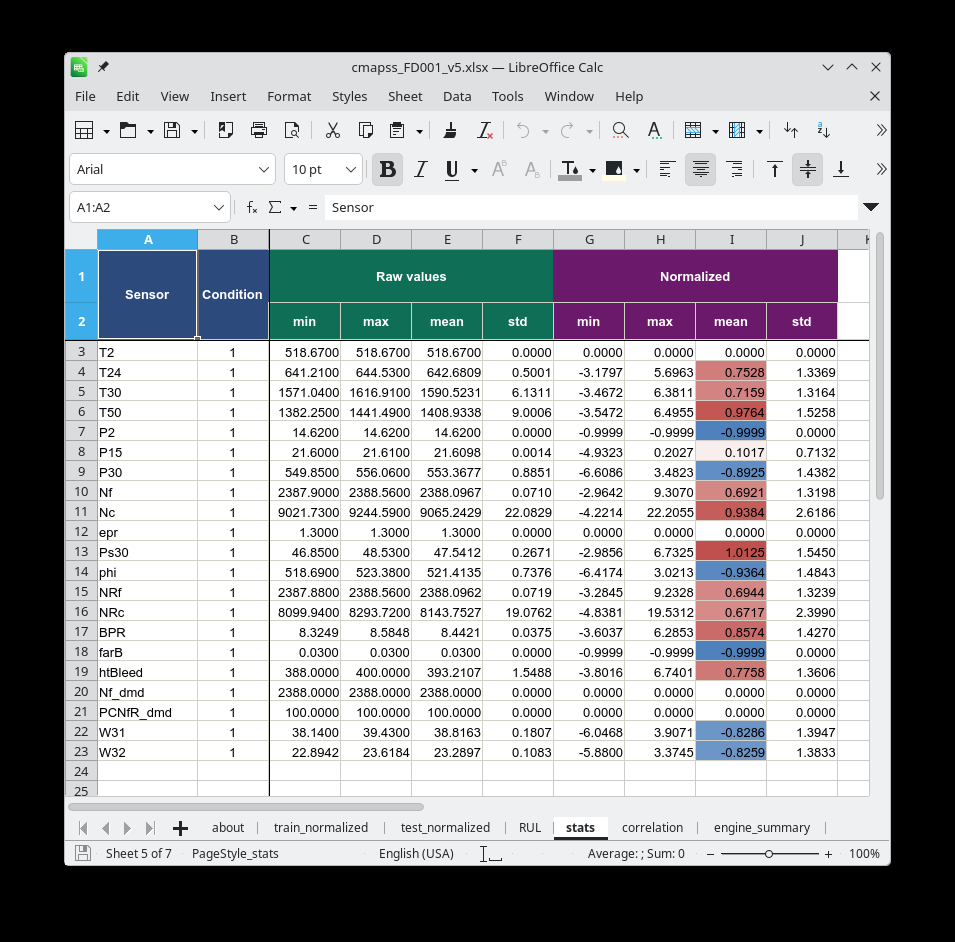
\includegraphics[width=\textwidth]{images/workbook-05-correlation-04-statistics.png}
    \caption{Sheet \texttt{stats} (v5) --- statistik raw dan ternormalisasi}
  \end{subfigure}
  \hfill
  \begin{subfigure}[b]{0.48\textwidth}
    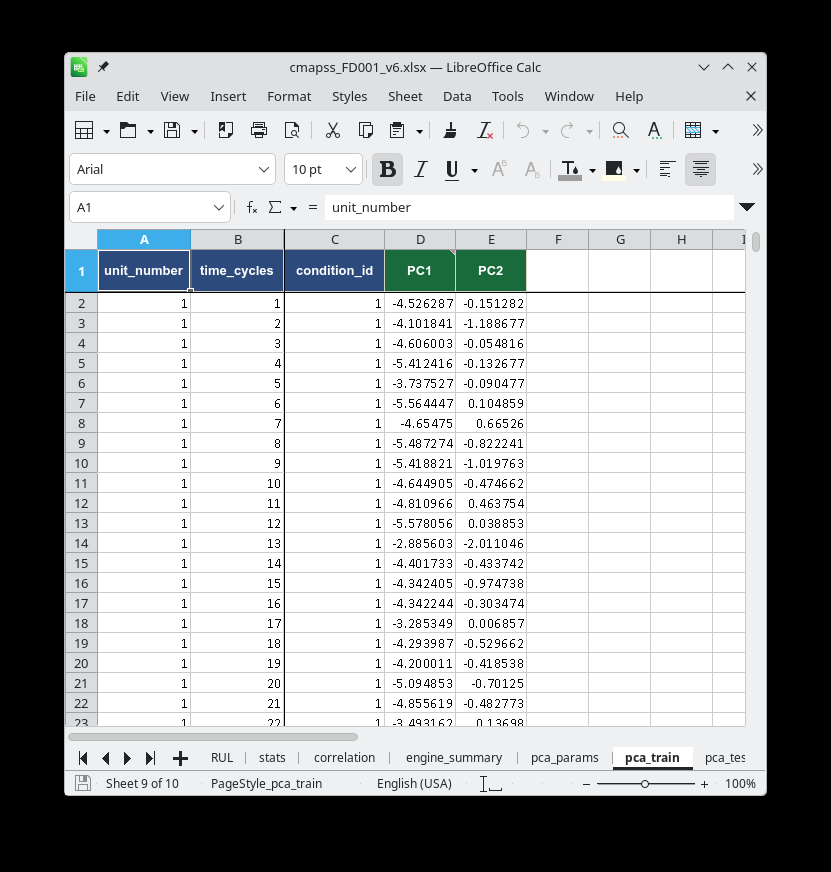
\includegraphics[width=\textwidth]{images/workbook-06-pca-12-pca-train.png}
    \caption{Sheet \texttt{pca\_train} (v6) --- skor PC per siklus}
  \end{subfigure}
  \caption{Contoh sheet spreadsheet v5 dan v6 (FD001)}
  \label{fig:spreadsheet}
\end{figure}

% ══════════════════════════════════════════════════════════════════════════════
\section{Model \textit{Artificial Neural Network}}

\subsection{Arsitektur MLP}

\begin{figure}[H]
  \centering
  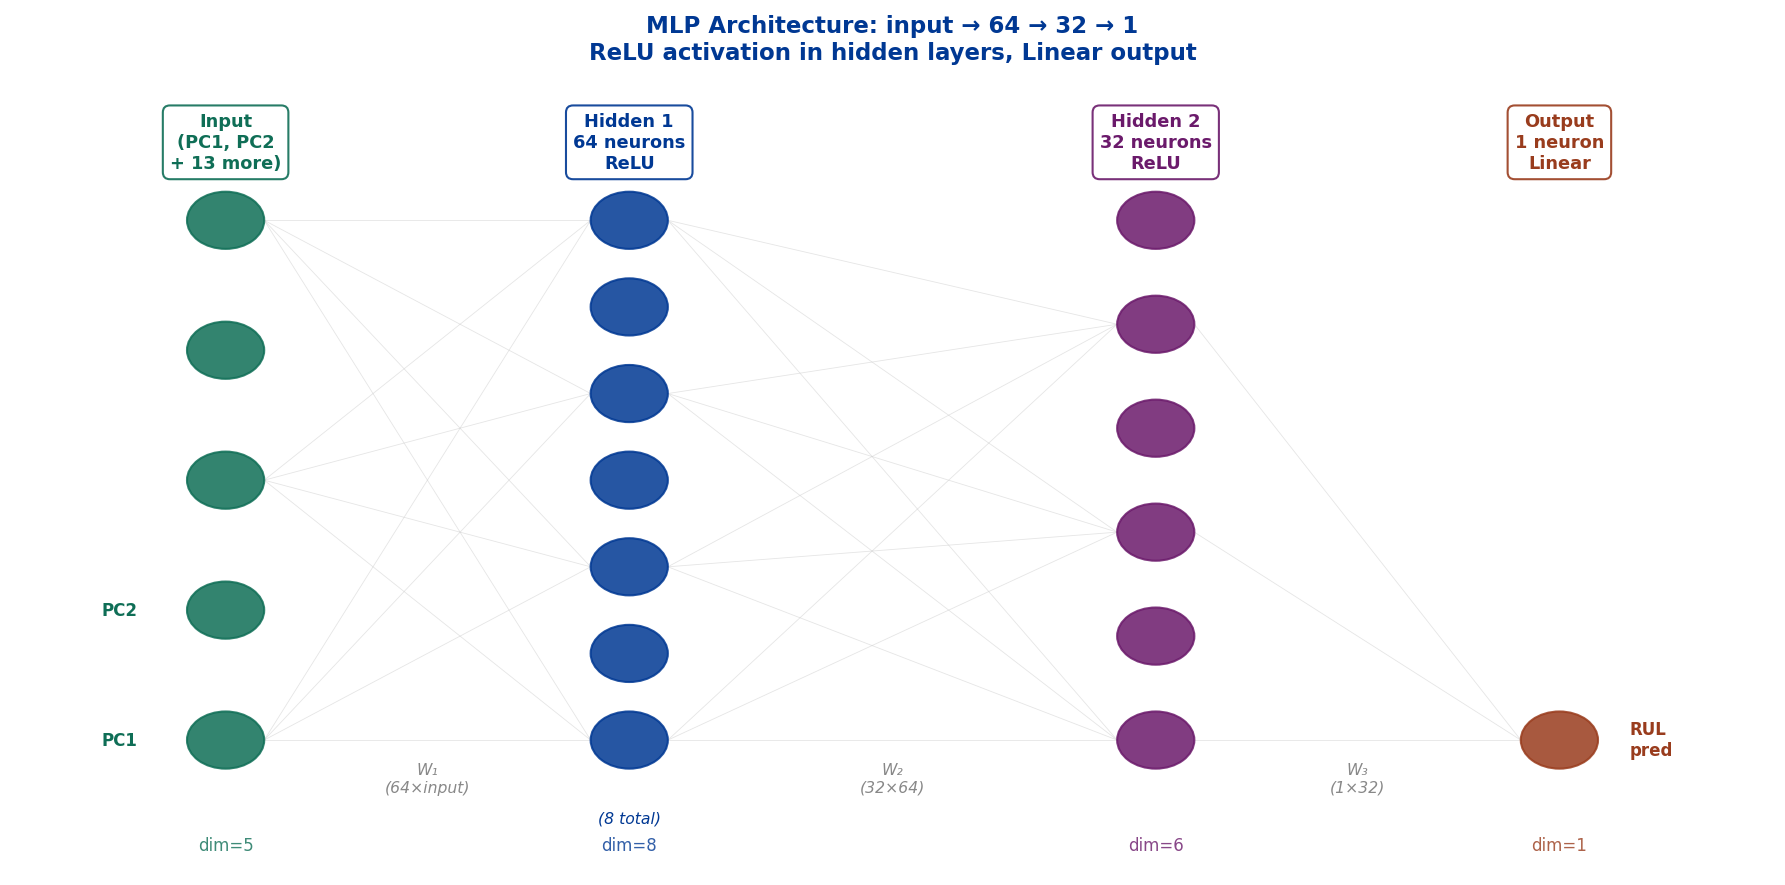
\includegraphics[width=0.88\textwidth]{images/plot_D14_mlp_arch.png}
  \caption{Arsitektur MLP yang digunakan --- tiga lapisan linear dengan
    aktivasi ReLU pada lapisan tersembunyi dan output linear;
    contoh input menunjukkan PC1 dan PC2 untuk model PCA}
  \label{fig:mlp_arch}
\end{figure}

Model \textit{Multilayer Perceptron} (MLP) dengan arsitektur tiga lapisan:
\begin{equation}
  \text{input} \xrightarrow{W_1,\,\text{ReLU}}
  64 \xrightarrow{W_2,\,\text{ReLU}}
  32 \xrightarrow{W_3}
  1
\end{equation}

\begin{table}[H]
\centering\small
\caption{Konfigurasi pelatihan ANN}
\label{tab:ann_config}
\begin{tabular}{ll}
\toprule
Parameter & Nilai \\
\midrule
Arsitektur    & input $\to$ 64 $\to$ 32 $\to$ 1 \\
Aktivasi      & ReLU (tersembunyi), Linear (output) \\
\textit{Loss} & MSE (\textit{Mean Squared Error}) \\
Optimizer     & Adam, lr $= 10^{-3}$ \\
Epoch         & 500 \\
Batch size    & 512 \\
Target        & RUL\_capped (cap $= 125$ siklus) \\
\bottomrule
\end{tabular}
\end{table}

\subsection{Target: RUL Capped}

\begin{figure}[H]
  \centering
  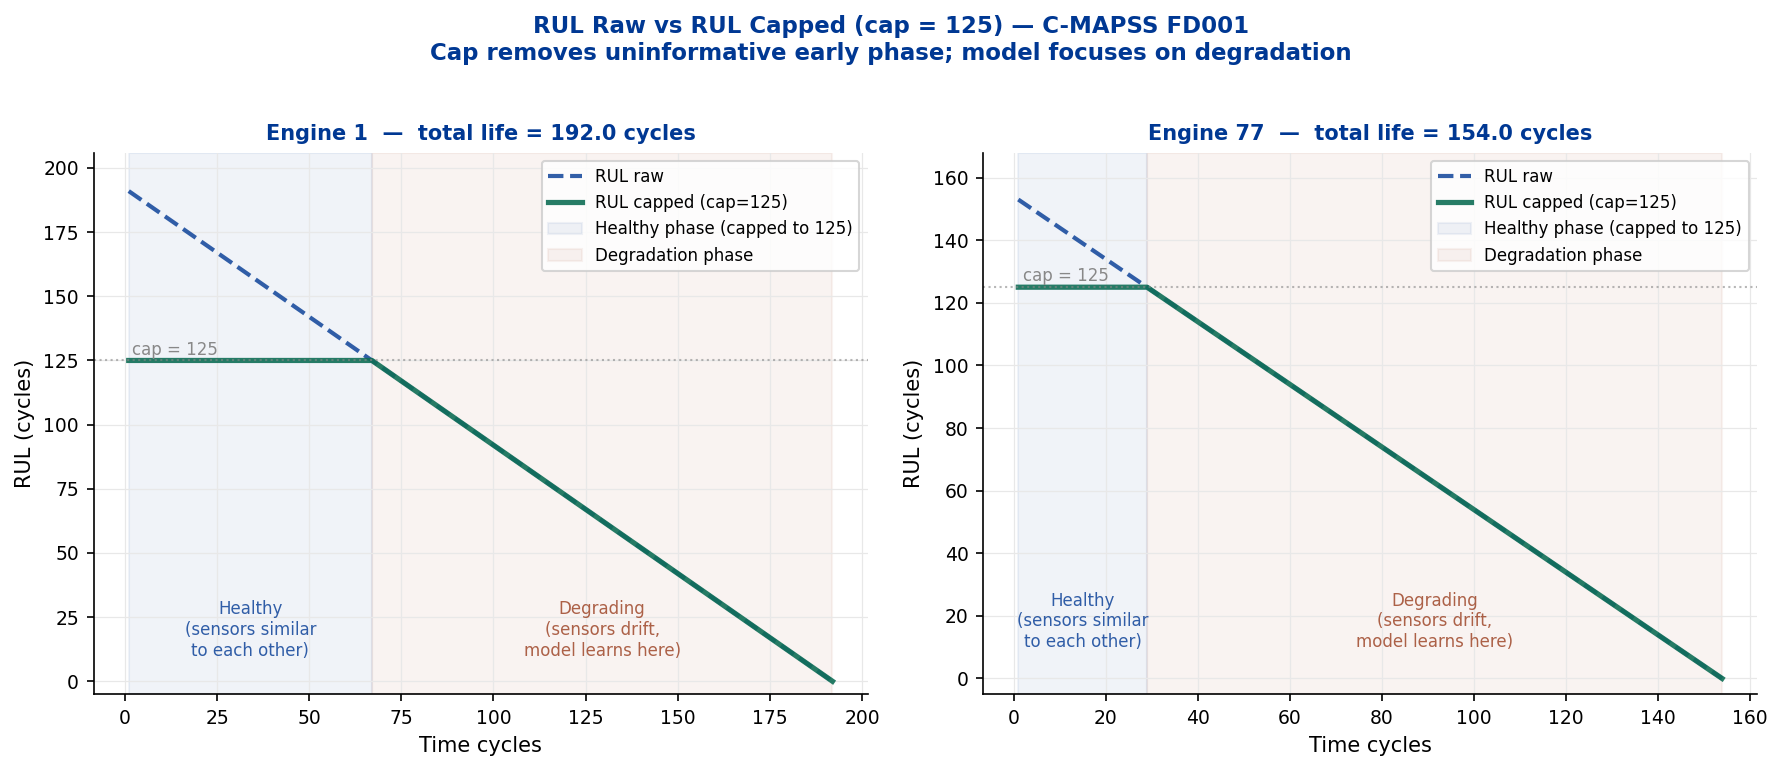
\includegraphics[width=0.90\textwidth]{images/plot_D12_rul_cap.png}
  \caption{RUL raw vs RUL capped (cap $= 125$) untuk dua mesin dengan
    umur total berbeda (Engine 1: 192 siklus, Engine 77: 154 siklus) ---
    fase sehat (biru) diratakan ke 125 pada kedua mesin;
    garis putus-putus menunjukkan kapan degradasi dimulai}
  \label{fig:rul_cap}
\end{figure}

Gambar \ref{fig:rul_cap} menunjukkan RUL raw (garis putus-putus biru)
dan RUL capped (garis solid teal) untuk dua mesin dengan total umur
berbeda. Dua mesin ditampilkan untuk membuktikan bahwa cap bekerja
\textit{konsisten} terlepas dari panjang hidup mesin: Engine 1
memasuki fase degradasi di siklus $\approx$67, sedangkan Engine 77
di siklus $\approx$29. Namun keduanya memiliki RUL\_capped $= 125$
selama fase sehat --- model memperlakukan semua mesin sehat secara
setara, dan baru belajar dari perbedaan sensor saat degradasi dimulai.

\subsection{Metrik Evaluasi}

Tiga metrik digunakan untuk evaluasi komprehensif:

\begin{itemize}[noitemsep]
  \item \textbf{RMSE} --- \textit{root mean square error}; sensitif
    terhadap \textit{outlier} karena error dikuadratkan
  \item \textbf{MAE} --- \textit{mean absolute error}; rata-rata
    error absolut, lebih robust terhadap \textit{outlier}
  \item \textbf{NASA Score} --- skor asimetris PHM08; prediksi
    \textit{late} dihukum lebih berat (Gambar \ref{fig:nasa_score})
\end{itemize}

\begin{figure}[H]
  \centering
  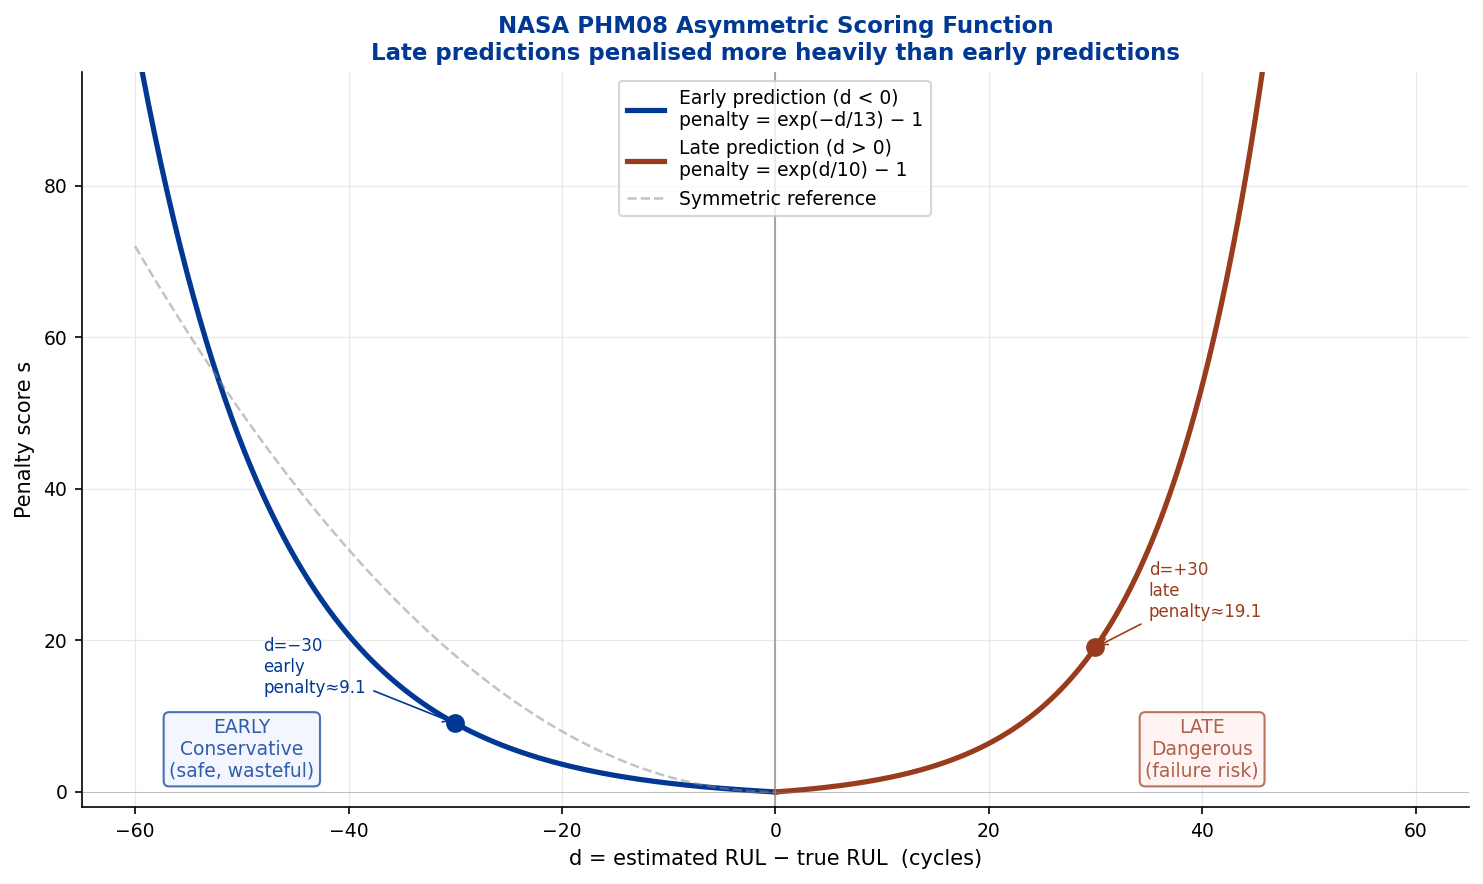
\includegraphics[width=0.80\textwidth]{images/plot_D11_nasa_score.png}
  \caption{Kurva penalti NASA Score --- prediksi \textit{early}
    ($d < 0$, biru, $e^{-d/13}-1$) dihukum lebih ringan dari prediksi
    \textit{late} ($d > 0$, merah, $e^{d/10}-1$) karena prediksi
    \textit{late} membahayakan keselamatan}
  \label{fig:nasa_score}
\end{figure}

Pada Gambar \ref{fig:nasa_score}, kurva merah (prediksi \textit{late})
memiliki kemiringan lebih curam dari kurva biru (prediksi \textit{early}).
Pada error $d = +30$ siklus (terlambat 30 siklus), penaltinya $\approx$10.
Namun pada $d = +50$ siklus, penaltinya sudah $\approx$47 --- meningkat
secara eksponensial. Ini mencerminkan realitas: memberitahu maskapai bahwa
mesin masih aman padahal sebenarnya hampir gagal adalah kesalahan yang
jauh lebih berbahaya dari sekadar jadwal perawatan yang terlalu konservatif.

\subsection{Desain Eksperimen Benchmark}

Benchmark dirancang sebagai eksperimen 2-faktor:
\textbf{Faktor 1} = sub-dataset (FD001--FD004);
\textbf{Faktor 2} = tipe input (PCA vs NORM).
Total 8 model dilatih dengan konfigurasi identik.

\subsection{Hasil Training}

\begin{figure}[H]
  \centering
  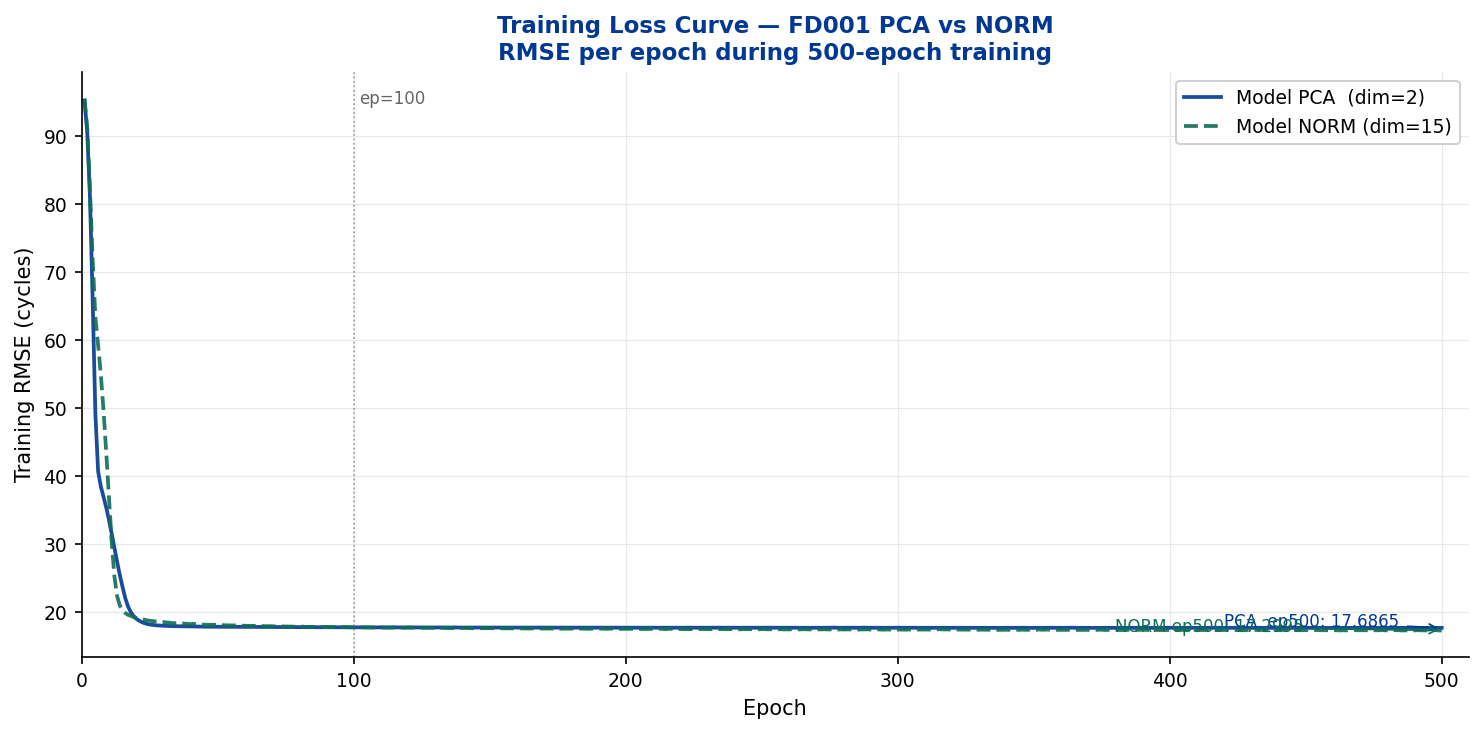
\includegraphics[width=0.88\textwidth]{images/plot_B5_loss_curve.png}
  \caption{Kurva \textit{loss} (training RMSE per epoch) untuk
    Model PCA (biru solid) dan Model NORM (teal putus-putus) FD001 ---
    PCA konvergen lebih cepat karena dimensi input lebih kecil
    (2 vs 15 fitur)}
  \label{fig:loss_curve}
\end{figure}

Gambar \ref{fig:loss_curve} menunjukkan kurva training RMSE selama
500 epoch. Model PCA (2 fitur) konvergen lebih cepat dan mendatar
sekitar epoch 200. Model NORM (15 fitur) masih perlahan menurun di
epoch 500 --- menunjukkan lebih banyak parameter yang perlu
dioptimalkan. Kedua model sudah konvergen dengan baik setelah 300 epoch.

\subsection{Hasil Benchmark}

\begin{table}[H]
\centering\small
\caption{Hasil benchmark 8 model (500 epoch, batch 512)}
\label{tab:benchmark}
\begin{tabular}{llcrrr}
\toprule
Sub-dataset & Input & Dim & RMSE & MAE & NASA Score \\
\midrule
FD001 & \textbf{PCA}  & 2  & \textbf{17,80} & \textbf{12,55} & \textbf{815} \\
FD001 & NORM & 15 & 18,21 & 13,52 & 929 \\
\midrule
FD002 & \textbf{PCA}  & 4  & \textbf{29,30} & \textbf{20,52} & 14.423 \\
FD002 & NORM & 21 & 29,45 & 20,73 & \textbf{12.990} \\
\midrule
FD003 & PCA  & 3  & 21,87 & 16,17 & 2.650 \\
FD003 & \textbf{NORM} & 16 & \textbf{20,16} & \textbf{15,28} & \textbf{1.783} \\
\midrule
FD004 & PCA  & 3  & 30,59 & 23,28 & 9.267 \\
FD004 & \textbf{NORM} & 21 & \textbf{29,68} & \textbf{22,38} & \textbf{7.157} \\
\bottomrule
\end{tabular}
\end{table}

\begin{figure}[H]
  \centering
  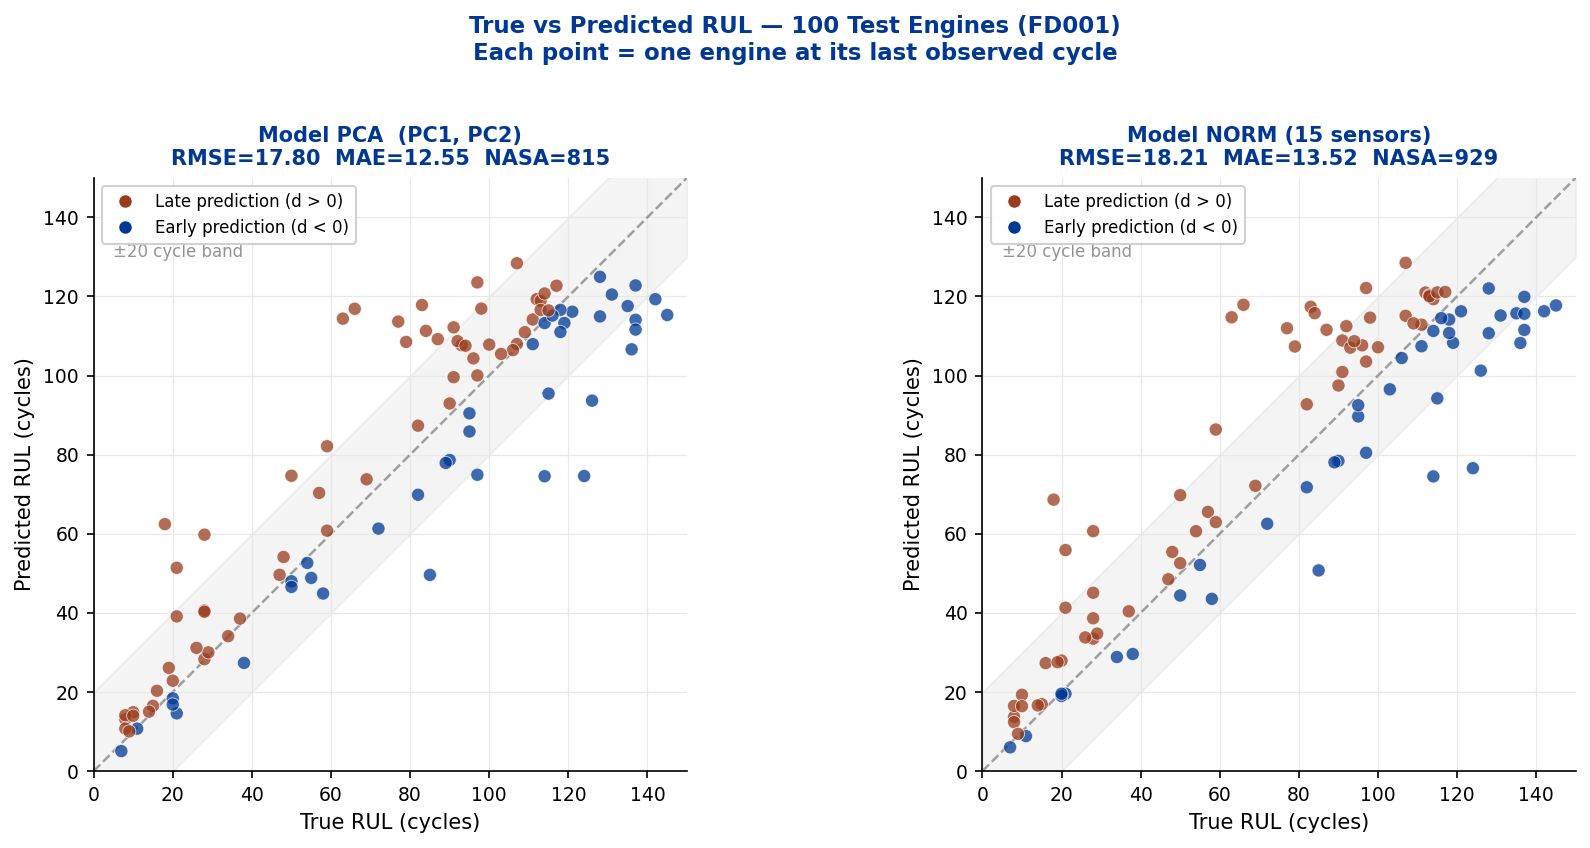
\includegraphics[width=0.90\textwidth]{images/plot_B6_true_vs_pred.png}
  \caption{True vs Predicted RUL untuk 100 mesin \textit{test} FD001 ---
    setiap titik adalah satu mesin pada siklus terakhir yang terobservasi;
    garis diagonal putus-putus = prediksi sempurna;
    titik merah = prediksi \textit{late} (di atas diagonal, berbahaya),
    titik biru = prediksi \textit{early} (di bawah diagonal, konservatif)}
  \label{fig:true_pred}
\end{figure}

Gambar \ref{fig:true_pred} menampilkan hasil prediksi untuk 100 mesin
\textit{test} FD001. Titik yang tepat pada diagonal berarti prediksi
sempurna. Titik di atas diagonal (merah) adalah prediksi \textit{late}
--- model mengatakan mesin masih punya lebih banyak siklus dari
kenyataannya. Pola linear (bukan kuadratik atau acak) muncul karena
RUL adalah \textit{countdown} linear --- target model juga linear,
sehingga hubungan prediksi vs aktual ikut menjadi linear.

\begin{figure}[H]
  \centering
  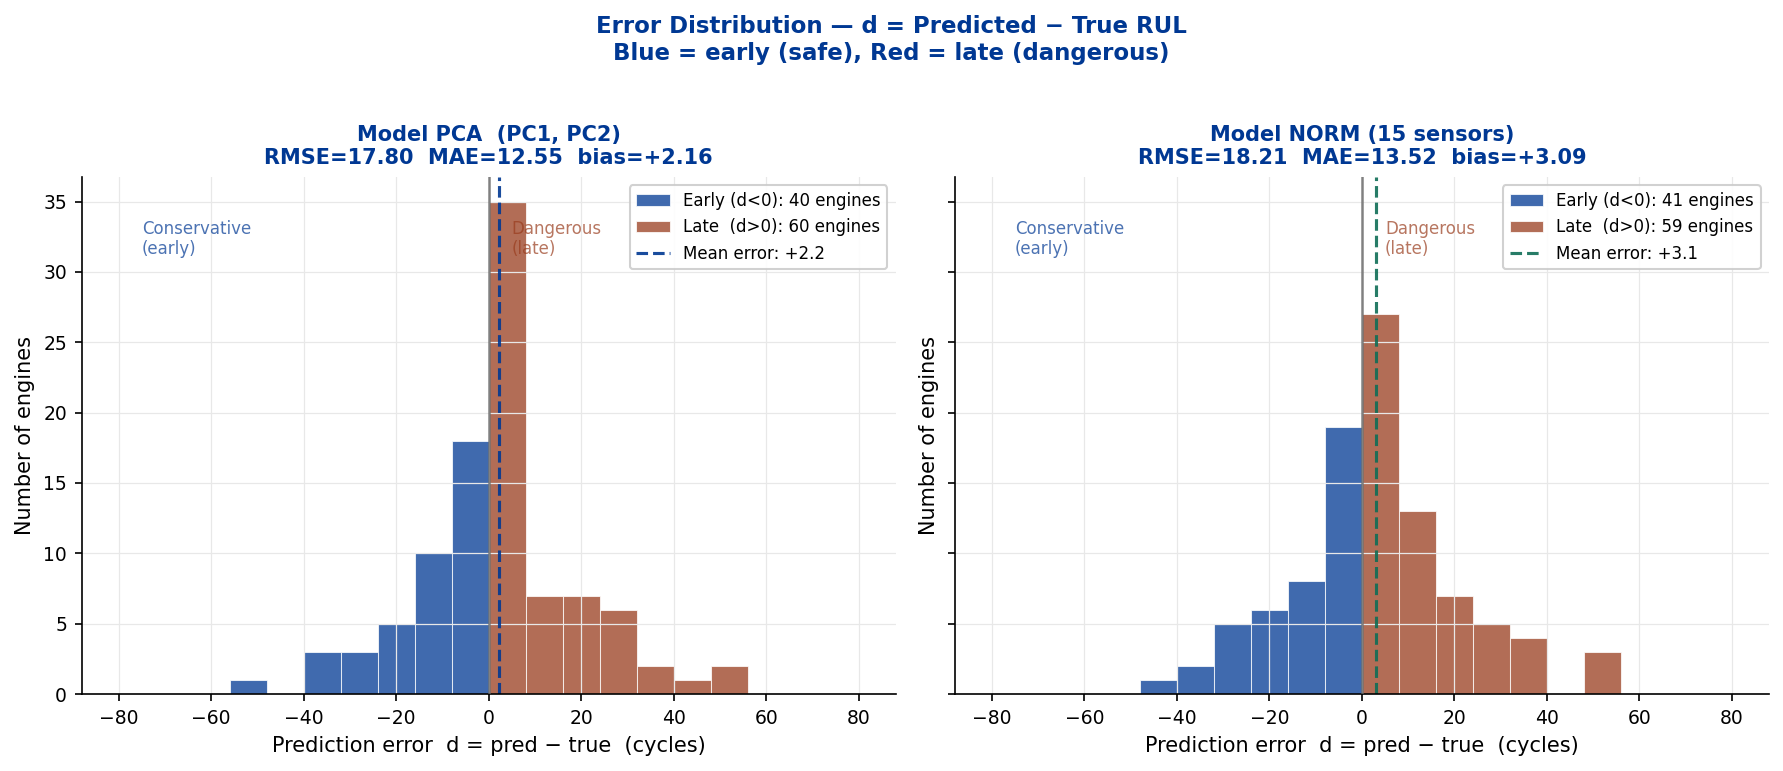
\includegraphics[width=0.90\textwidth]{images/plot_B7_error_dist.png}
  \caption{Distribusi error prediksi ($d = \text{pred} - \text{true}$)
    untuk 100 mesin test FD001 --- distribusi \textit{right-skewed}
    pada kedua model menunjukkan bias \textit{late prediction};
    garis putus-putus vertikal = mean error (bias)}
  \label{fig:error_dist}
\end{figure}

Gambar \ref{fig:error_dist} menunjukkan histogram error. Kedua model
memiliki distribusi yang \textit{right-skewed} --- lebih banyak mesin
dengan error positif (\textit{late}) dari pada negatif (\textit{early}).
Model PCA memiliki distribusi lebih sempit dan bias lebih kecil, yang
menjelaskan NASA Score yang lebih rendah (815 vs 929).

\subsection{Analisis Faktor}

\textbf{Faktor 1 --- Kompleksitas sub-dataset} adalah faktor dominan.
Sub-dataset 6 kondisi (FD002, FD004) menghasilkan RMSE $\approx 60\%$
lebih tinggi ($\approx$30) dibandingkan 1 kondisi ($\approx$18--21).

\textbf{Faktor 2 --- Tipe input} menunjukkan interaksi dengan Faktor 1:
PCA lebih baik pada FD001/FD002 (1 kondisi atau sederhana), sedangkan
NORM lebih baik pada FD003/FD004 (kompleks). Kompresi PCA efektif
membuang \textit{noise} pada dataset sederhana, namun membuang informasi
yang relevan pada dataset kompleks.

% ══════════════════════════════════════════════════════════════════════════════
\section{Analisis Garson}

\subsection{Algoritma}

Algoritma Garson \cite{garson1991} menghitung kepentingan relatif
fitur input berdasarkan bobot jaringan terlatih. Untuk arsitektur
dua lapisan tersembunyi ($W_1$, $W_2$, $W_3$):

\begin{align}
  q_1[i,j] &= \frac{|W_1[j,i]|}{\sum_k |W_1[j,k]|} &
  q_2[j,m] &= \frac{|W_2[m,j]|}{\sum_k |W_2[m,k]|} \\[4pt]
  r[i,m]   &= \sum_j q_1[i,j] \cdot q_2[j,m] &
  s[i]     &= \sum_m r[i,m] \cdot |W_3[m]| \\[4pt]
  \text{importance}[i] &= \frac{s[i]}{\sum_k s[k]}
\end{align}

Hasil adalah satu skor kepentingan per fitur, total 100\%.

\subsection{Model PCA --- Kepentingan Komponen}

\begin{figure}[H]
  \centering
  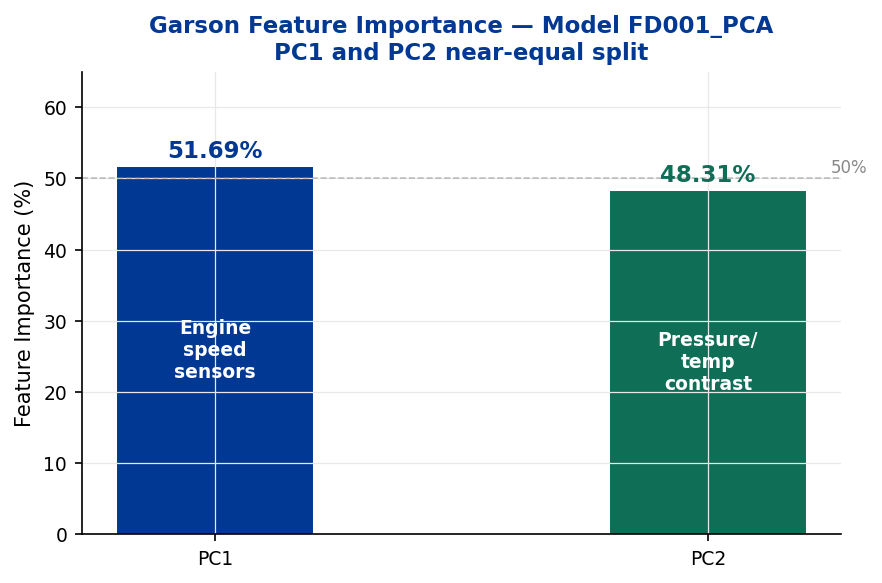
\includegraphics[width=0.55\textwidth]{images/plot_C10_garson_pca.png}
  \caption{Kepentingan Garson untuk Model FD001\_PCA ---
    PC1 (kecepatan mesin) dan PC2 (kontras tekanan-kecepatan)
    hampir seimbang di 51,69\% vs 48,31\%}
  \label{fig:garson_pca}
\end{figure}

Model PCA menunjukkan pembagian yang hampir sempurna 50-50 antara
PC1 dan PC2. Ini berarti model ANN menggunakan kedua komponen secara
setara --- PC1 (yang merepresentasikan kecepatan mesin) dan PC2
(yang merepresentasikan kontras tekanan-kecepatan) sama-sama penting
untuk prediksi RUL yang akurat.

\subsection{Model NORM --- Kepentingan Sensor}

\begin{figure}[H]
  \centering
  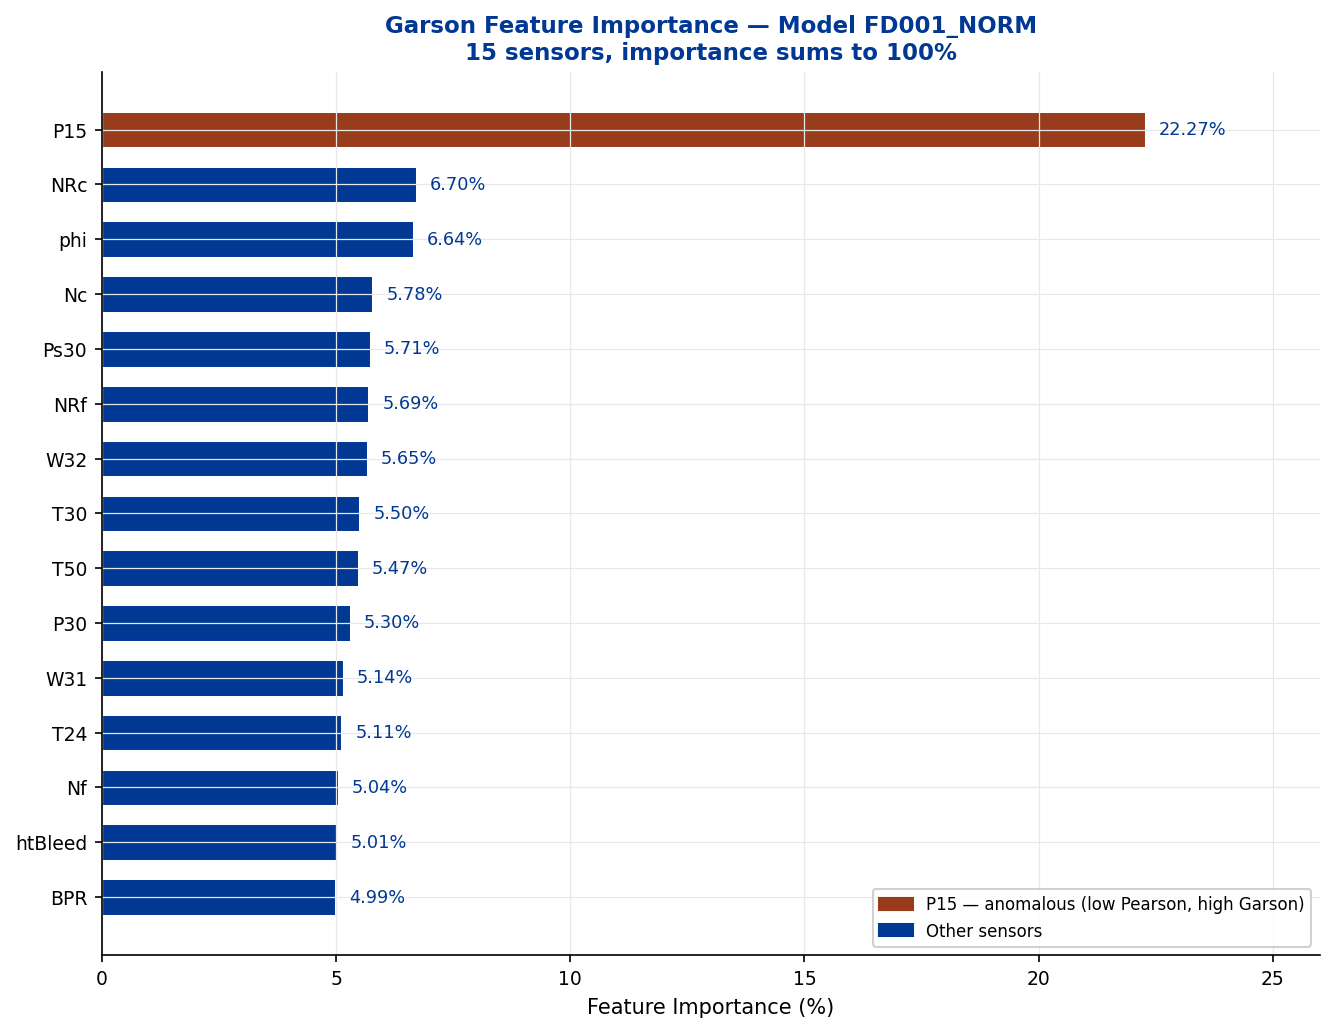
\includegraphics[width=0.88\textwidth]{images/plot_C8_garson_norm.png}
  \caption{Kepentingan Garson untuk 15 sensor Model FD001\_NORM ---
    P15 mendominasi dengan 22,27\% meskipun korelasi Pearson-nya
    hanya $-0{,}13$; batang merah = sensor anomali P15}
  \label{fig:garson_norm}
\end{figure}

Gambar \ref{fig:garson_norm} menunjukkan hasil yang mengejutkan:
sensor \textbf{P15} mendominasi dengan 22,27\% --- lebih dari 3$\times$
sensor terpenting berikutnya (NRc 6,70\%). Hal ini mengejutkan karena
korelasi Pearson P15 terhadap RUL hanya $-0{,}13$ (hampir tidak ada
hubungan linear). ANN menemukan hubungan \textit{non-linear} yang tidak
terdeteksi oleh metode linear.

\subsection{Perbandingan Tiga Metode}

\begin{figure}[H]
  \centering
  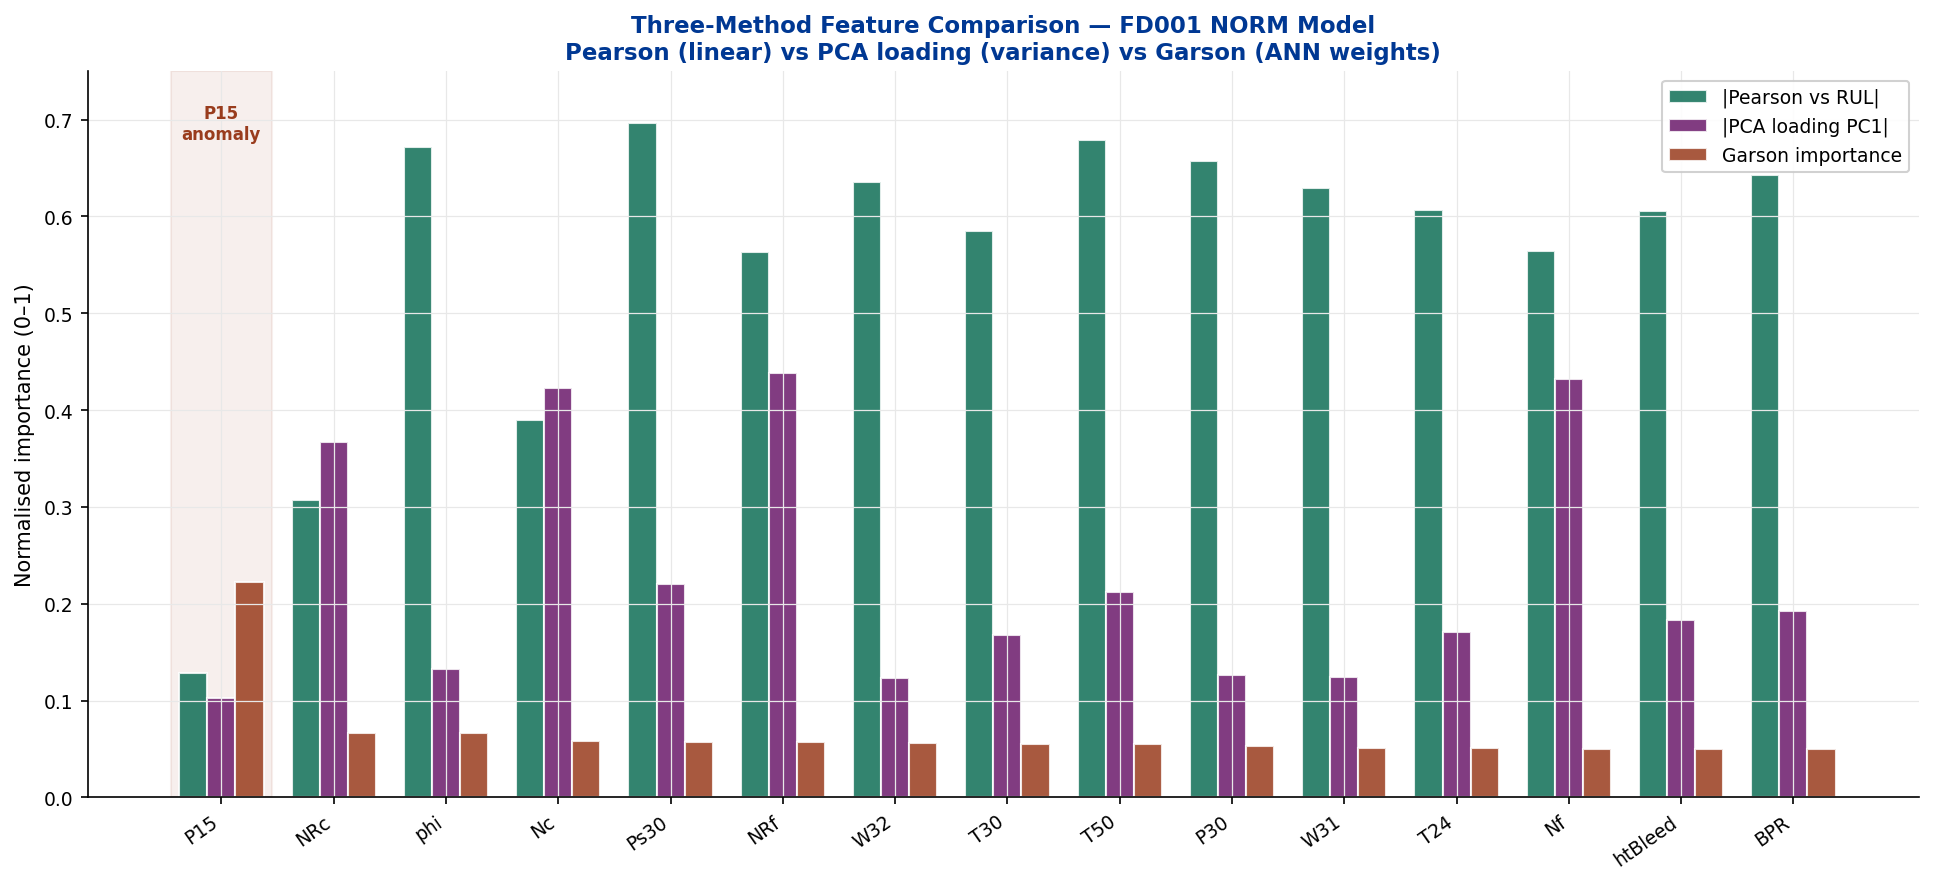
\includegraphics[width=0.95\textwidth]{images/plot_C9_three_method.png}
  \caption{Perbandingan kepentingan sensor menggunakan tiga metode
    (FD001 NORM model) --- teal = $|$Pearson vs RUL$|$,
    ungu = $|$PCA loading PC1$|$, merah = Garson importance;
    area diarsir kuning = anomali P15 yang hanya terdeteksi Garson}
  \label{fig:three_method}
\end{figure}

Gambar \ref{fig:three_method} adalah visualisasi paling penting
dalam laporan ini. Untuk sensor P15 (diarsir kuning): batang teal
(Pearson) hampir tidak terlihat, batang ungu (PCA) juga sangat kecil,
namun batang merah (Garson) jauh lebih tinggi dari semua sensor lain.
Ini adalah bukti visual bahwa ANN menemukan pola non-linear yang tidak
dapat dideteksi oleh dua metode seleksi fitur berbasis statistik linear.

\begin{table}[H]
\centering\small
\caption{Perbandingan tiga metode untuk sensor pilihan (FD001)}
\label{tab:three_method}
\begin{tabular}{lcccp{5cm}}
\toprule
Sensor & Pearson & PCA Loading & Garson & Interpretasi \\
\midrule
Ps30   & $-0{,}70$ & tinggi & sedang
  & Konsisten --- penting secara linear \\
T50    & $-0{,}68$ & tinggi & sedang
  & Konsisten --- penting secara linear \\
P30    & $+0{,}66$ & tinggi & sedang
  & Konsisten --- penting secara linear \\
\textbf{P15}
       & $-0{,}13$ & rendah & \textbf{22,27\%}
  & \textbf{Anomali} --- ANN menemukan sinyal non-linear \\
NRf    & $-0{,}56$ & sedang & rendah
  & Sebagian konsisten \\
\bottomrule
\end{tabular}
\end{table}

% ══════════════════════════════════════════════════════════════════════════════
\section{Keterbatasan dan Pengembangan}

\subsection{Keterbatasan}

\begin{enumerate}[noitemsep]
  \item \textbf{Arsitektur MLP sederhana}: setiap siklus diperlakukan
    independen tanpa memanfaatkan dependensi temporal
  \item \textbf{Dataset simulasi}: C-MAPSS adalah data simulasi;
    degradasi mesin nyata lebih kompleks dan tidak se-linear ini
  \item \textbf{Tanpa regularisasi}: tidak ada \textit{dropout};
    gap antara train RMSE dan test RMSE mengindikasikan \textit{overfitting} ringan
  \item \textbf{Garson untuk dua lapisan}: algoritma Garson orisinal
    dirancang untuk satu lapisan tersembunyi; ekstensi ke dua lapisan
    kurang didukung literatur
\end{enumerate}

\subsection{Pengembangan yang Memungkinkan}

\begin{enumerate}[noitemsep]
  \item \textbf{LSTM/GRU}: memanfaatkan urutan temporal siklus
  \item \textbf{Dropout}: mengurangi \textit{overfitting}
  \item \textbf{Normalisasi per kondisi lebih ketat}: terutama untuk
    FD002/FD004 yang memiliki 6 kondisi operasi
\end{enumerate}

% ══════════════════════════════════════════════════════════════════════════════
\section{Kesimpulan}

\begin{enumerate}[noitemsep]
  \item \textbf{Kompleksitas kondisi operasi adalah faktor dominan}.
    Sub-dataset 6 kondisi (FD002, FD004) menghasilkan RMSE $\approx$60\%
    lebih tinggi dari sub-dataset 1 kondisi, terlepas dari tipe input.

  \item \textbf{Tipe input optimal bergantung pada kompleksitas dataset}.
    PCA lebih baik untuk dataset sederhana (1 kondisi); sensor penuh
    lebih baik untuk dataset kompleks (6 kondisi atau 2 mode kerusakan).

  \item \textbf{Normalisasi healthy-only per kondisi mempertahankan
    sinyal degradasi}. Terbukti dari Gambar \ref{fig:norm_comparison}:
    ketiga mesin mulai di $z \approx 0$ dan secara konsisten
    \textit{drift} seiring degradasi.

  \item \textbf{Algoritma Garson mengungkap hubungan non-linear}.
    Sensor P15 --- Pearson rendah, PCA loading rendah ---
    terbukti menjadi fitur terpenting menurut Garson (22,27\%),
    menunjukkan ANN mengeksploitasi pola yang tidak terdeteksi
    metode linear.

  \item \textbf{Eliminasi sensor harus per sub-dataset}.
    Sensor konstan di FD001 (T2, P2) menjadi fitur aktif di FD002
    karena variasi antar kondisi operasi mengandung informasi degradasi.
\end{enumerate}

% ── References ────────────────────────────────────────────────────────────────
\begin{thebibliography}{9}
\bibitem{saxena2008}
  A. Saxena, K. Goebel, D. Simon, N. Eklund,
  ``Damage Propagation Modeling for Aircraft Engine Run-to-Failure Simulation,''
  \textit{Proc.\ 1st Int.\ Conf.\ Prognostics and Health Management (PHM08)},
  Denver, CO, 2008.

\bibitem{garson1991}
  G.D. Garson,
  ``Interpreting Neural Network Connection Weights,''
  \textit{AI Expert}, vol.~6, no.~4, pp.~46--51, 1991.
\end{thebibliography}

\end{document}
